\documentclass{article}
\usepackage{microtype}
\usepackage{graphicx}
\usepackage{subcaption}
\usepackage{booktabs}
\usepackage{xurl}
\usepackage{hyperref}
\usepackage[T1]{fontenc}
\usepackage{icml2026}
\usepackage{amsmath,amssymb,amsfonts,mathtools}
\usepackage{amsthm}
\usepackage{placeins}
\usepackage[nameinlink,capitalize,noabbrev]{cleveref}
\newcommand{\R}{\mathbb{R}}
\newcommand{\Id}{\mathbf{I}}
\newcommand{\norm}[1]{\left\lVert #1\right\rVert}
\newcommand{\Eeq}{E_{\mathrm{eq}}}
\newcommand{\Ehom}{E_{\mathrm{hom,data}}}
\newcommand{\Ehomop}{E_{\mathrm{hom,op}}}
\newcommand{\Erel}{E_{\mathrm{rel,data}}}
\newcommand{\Erelop}{E_{\mathrm{rel,op}}}
\newcommand{\Ecomp}{E_{\mathrm{comp,data}}}
\newcommand{\Ecompop}{E_{\mathrm{comp,op}}}
\newtheorem{proposition}{Proposition}
\newtheorem{corollary}[proposition]{Corollary}
\icmltitlerunning{What Finite-Group Recovery Identifies}
\begin{document}
\twocolumn[
\icmltitle{Beyond Shared Geometry: What Do Recovered Group Actions Identify in Language Models?}
\begin{icmlauthorlist}
\icmlauthor{Anonymous Authors}{anon}
\end{icmlauthorlist}
\icmlaffiliation{anon}{Anonymous Institution}
\icmlcorrespondingauthor{Anonymous Authors}{anonymous@example.com}
\icmlkeywords{representation learning, group actions, equivariance, mechanistic interpretability}
\vskip 0.3in
]
\printAffiliationsAndNotice{}

\begin{abstract}
What do recovered group actions establish about language-model representations? We examine weekday cycles ($C_7$) and square-corner actions ($D_4$) across six pretrained models. Independent linear operators attain held-out squared relative prediction errors near 0.05, and generator-only fits predict excluded action elements on the same state vocabulary. The completed controls reveal three findings. Predictive recovery coexists with competitive category and coherently registered alternatives. Predictor rankings depend on storage: the tested RFF and Nystr\"om models do not improve panel means at the linear reference budget, but do at larger budgets. Directly fitting contextual differences reduces transport loss relative to applying coordinate-fitted operators, while a coherent alternative correspondence yields close means. Elementary realization and error-propagation identities explain why positive recovery diagnostics alone do not resolve these alternatives. Together, the results characterize predictive action structure, estimator tradeoffs and contextual transport on a fixed panel. They support recovery across the declared contexts, while leaving preferential semantic alignment and native causal implementation unresolved.
\end{abstract}

\section{Introduction}
Which additional interpretation is justified when a fitted transformation predicts well, approximately obeys group laws, and outperforms disrupted correspondences? These tests may appear to reinforce one another, yet they address different questions. A useful predictor is not by itself an account of a model's computation; consistency can follow partly from accurate prediction; disrupting a registration does not test whether the specified semantic correspondence is uniquely favored. We study these distinctions through controlled finite actions in contextual language-model representations.

Transformation fitting is established: \citet{lenc2015understanding} study paired maps and network stitching, and \citet{sun2026transformationlaws} develops compatible transformation families, realizability and transport. Equivariance by Contrast identifies jointly learned coordinates and actions under explicit assumptions \citep{schmidt2025equivariance}. Calendar mechanisms are studied by \citet{engels2025notall}; group-operation mechanisms and competing explanations by \citet{nanda2023progress,chughtai2023toy,wu2025unified}. Implementation-family equivalence requires abstraction assumptions \citep{sun2026tracking}. We test which identification claims finite-action controls support; \cref{app:related-work} gives the comparisons.

The protocol fits shared operators to activations of seven weekday states and four corner states across held-out short templates. States are visible in the input, and the language models remain unchanged. Independent fitting removes group-law penalties from the objective, while generator-only fitting withholds action elements. Both succeed predictively. We then compare category predictors, a coherently registered alternative action, compact nonlinear predictors and context-difference fits to determine what these successes distinguish.

Our empirical contribution is threefold. First, predictive transfer across held-out templates and excluded action elements coexists with alternatives that disrupted-registration and training-correspondence controls do not exclude. Second, predictor rankings change with the declared storage budget; the label-informed category control also improves the $C_7$ mean without winning in most cells. Third, fitting contextual differences directly improves transport, while the tested coherent alternative still gives close descriptive means. The analytical results explain limits of interpreting these observations as semantic identification. This fixed-panel account of predictive structure and competing explanations, summarized in \cref{tab:identification-summary}, is our contribution within the established transformation-recovery literature.

% Generated by scripts/build_identification_table.py; see identification_summary.source.json.
\begin{table*}[t]
\centering\small
\setlength{\tabcolsep}{4pt}
\renewcommand{\arraystretch}{1.10}
\begin{tabular}{@{}p{.16\textwidth}p{.40\textwidth}p{.40\textwidth}@{}}
\toprule
Test and endpoint & Recorded observation ($C_7$ / $D_4$) & Supported conclusion and remaining alternative \\
\midrule
Independent fits\newline (FULL, $D$) & Ridge: 0.04830 / 0.05200. & Shared linear maps predict activations in held-out templates; stable category coding remains compatible. \\
\addlinespace[3pt]
Generator transfer\newline (AFS-A, $D$) & Composed: 0.074443 / 0.056558. \newline Direct: 0.051124 / 0.050032. & Transfer to five excluded action elements; state labels remain seen. Direct fits receive additional element supervision. \\
\addlinespace[3pt]
Context differences\newline (replay transport) & Coordinate fit: 0.047137 / 0.132304. \newline Direct fit: 0.034260 / 0.116386. \newline Coherent fit: 0.034465 / 0.117165. & Direct fitting helps; a coherent alternative has close means. Targets and masks are registration-specific; closeness is not equivalence. \\
\addlinespace[3pt]
Compact nonlinear\newline (replay prediction) & First tested budget with lower mean than ridge, in both groups:\newline Nystr\"om $2\times$; RFF $4\times$. & Predictor ranking depends on storage. Parameter bytes do not match statistical capacity or runtime. \\
\addlinespace[3pt]
Category control\newline (replay prediction) & Centroid: 0.012013 / 0.063821. \newline Ridge: 0.014897 / 0.041919. \newline Centroid lower in 9/24 / 2/24 cells. & Category coding is competitive for the C7 mean, not most cells; centroids receive extra training labels and the action table. \\
\addlinespace[3pt]
Restricted registration\newline (AFS-B) & 120/120 cells in each group, separately for data and operator defects, below the reference 2.5th percentile. & Separation from invalid registrations; the restricted ensemble is not a calibrated semantic null. \\
\bottomrule
\end{tabular}
\caption{Evidence and identification boundaries. Paired numbers are $C_7$ / $D_4$ (corners); smaller losses are better. Rows concern different experiments, not one matched comparison or independent confirmations. Historical $D$ averages per-row target-normalized squared errors; replay prediction and context transport use distinct training-energy denominators $E_z$ and $E_u$. Compare losses only within the stated study and endpoint. Replay means cover 24 fixed model/readout cells per group. Budget crossovers are descriptive across the full recorded grid, not a test-selected deployment policy. D4 fixed-point identities, and hence scored rows, can differ across registrations. Statistical scope is defined in Section~\ref{sec:setup}.}
\label{tab:identification-summary}
\end{table*}


\section{Protocol and Evidence Scope}
\label{sec:setup}
Let $G$ act on states $i$, and let $t$ index contextual templates. For each model, layer, and split, training activations determine mean $\mu$ and orthonormal PCA columns $C\in\R^{d\times q}$. We use
\begin{equation}
 z_{i,t}=(h_{i,t}-\mu)C,\qquad z_{i,t}R_g\approx z_{g(i),t}.
\end{equation}
For row vectors, applying $g_2$ then $g_1$ gives
\begin{equation}
 R_{g_2}R_{g_1}\approx R_{g_1\circ g_2}.
 \label{eq:convention}
\end{equation}
The primary dimension is $q=16$. AFS-D uses matched $q=6$ for seven weekdays and $q=3$ for four corners.

\paragraph{Estimation.}
Ridge fits each element independently, without an intercept, using regularization $\alpha=0.01$. Joint fitting starts from ridge: the data term has coefficient one, and the homomorphism, relation, identity and orthogonality penalties have coefficients $1,1,1,0.05$, respectively. AdamW runs for 1,200 steps, learning rate $0.002$, weight decay $10^{-5}$, and technical seed 42. All transformations use the same fixed training-only PCA. Full objectives appear in \cref{app:methods}.

\paragraph{Evaluation.}
For paired row matrices define
\begin{equation}
 D(A,B)=\frac{1}{m}\sum_{j=1}^m
 \frac{\norm{A_j-B_j}_2^2}{\norm{B_j}_2^2+10^{-12}}.
 \label{eq:D}
\end{equation}
$\Eeq$ averages $D(ZR_g,Z_g)$ over nonidentity actions on held-out templates. $\Ehom$ averages $D(ZR_{g_2}R_{g_1},ZR_{g_1\circ g_2})$ over element pairs. $\Ecomp$ uses the same expression excluding pairs containing the identity; it is a restricted consistency summary, not an independent unseen-element test. AFS-A instead compares generator products with \emph{actual} held-out transformed activations. Relation and operator-space definitions are explicit in \cref{app:metrics}. Data defects are squared relative errors, whereas the reported homomorphism, composition, and relation operator diagnostics use unsquared relative Frobenius norms. Their raw magnitudes cannot be directly compared.

\paragraph{Panel and partitions.}
\label{sec:design}
We use pretrained base Llama-3.2-1B/3B, Llama-3.1-8B, and Qwen2.5-1.5B/3B/7B models at normalized depth slots $0.2,0.4,0.6,0.8$. The $C_7$ action cycles Monday through Sunday. The $D_4$ action rotates and reflects the labels NW, NE, SE, SW. Each domain contains 40 short templates, such as ``The current day is Monday.'' and ``The marked corner is NW.'' The state is visible in the input; no held-out vocabulary, unseen semantic domain, or abstract reasoning task is tested.

For each of five split seeds $(101,303,909,2701,4243)$, 28 templates train PCA and operators, six are diagnostic validation templates, and six are test templates. Complete state orbits stay within their template split. The same 40 templates recur across splits; the seeds represent repeated partitions, not five independently sampled datasets. Activations are mean hidden states over the unique lexical target-token span at transformer block outputs. Exact model revisions, tokenization, layers, prompts, and sensitivity subsets are in \cref{app:methods}.

The evidence comprises a structural recovery panel (FULL and AFS) and subsequent predictor and context-transport comparisons. FULL compares ridge, joint, identity and random controls; AFS tests generator products, disrupted correspondences and rank-matched lexical codes. Later comparisons use separate training-energy normalizations. The appendices map these experiments to their source records, full estimates and preserved stopping decisions.

\paragraph{Statistical scope.}
All comparisons in this paper are descriptive analyses of the recorded fixed panels. Computational replay re-executes inspected designs and supplies no independent confirmation. We retain the recorded means and bootstrap percentile intervals. Historical FULL uses 5,000 draws, base seed 314159 with analysis-specific offsets, and model, depth, split, and template levels, adding random-control seed where relevant. AFS-D keeps depth fixed for its matched contrasts; the separate global-additive experiment resamples split aggregates. The six models are deliberately selected, layers are repeated measurements, and template partitions overlap. These intervals describe resampling sensitivity under the recorded scheme; nominal 95\% does not assert calibrated population coverage. Numerous secondary intervals are not globally multiplicity-adjusted. We make no new significance or equivalence decisions from them; \cref{app:inference} gives their scope.

\section{Why Positive Recovery Does Not Settle Identification}
\label{sec:boundaries}
The following elementary facts delimit the empirical claims. They specialize standard realization and perturbation arguments to our finite-state protocol; the broader induced-action and accumulation questions are developed by \citet{sun2026transformationlaws}. Proofs and further coordinate/context diagnostics appear in \cref{app:theory}.

Measured predictor performance, the best risk in a specified function class, an exact action on supported features, and the model's native mechanism are distinct targets. A successful fit witnesses predictability under its information and evaluation conditions; failure of selected fits does not exclude other maps in a larger class. Under exact realizability, the observed states determine a linear action only on their span. Its extension beyond that span and its internal implementation remain separate questions (\cref{app:contextual-realization,app:coordinates}).

\paragraph{Finite states can support exact algebra automatically.}
\begin{proposition}[Finite-orbit realizability]
\label{prop:finite}
Let $X\in\R^{n\times(n-1)}$ have centered rows and rank $n-1$. For a permutation $g$, define $(P_gX)_i=X_{g(i)}$. There is a unique invertible $R_g=X^\dagger P_gX$ satisfying $XR_g=P_gX$, and $R_gR_h=R_{h\circ g}$.
\end{proposition}
Thus seven generic centered lexical vectors in six dimensions realize a weekday cycle exactly; four generic centered vectors in three dimensions realize every corner permutation, including $D_4$. This is a conjugated permutation representation, not evidence that a model learned the named group's semantics. Separate contextual orbits need not share one realization; a conjugacy counterexample is given in \cref{app:theory}. Conversely, a stable state code plus context features in an invariant complementary subspace \emph{can} share a realization. Held-out templates alone do not exclude this alternative.

\paragraph{Prediction already constrains composition.}
Write $e_g(i,t)=z_{i,t}R_g-z_{g(i),t}$.
\begin{proposition}[Prediction-error propagation]
\label{prop:propagation}
For $p=g_1\circ g_2$, the composition residual is
\begin{align}
 z_{i,t}(R_{g_2}R_{g_1}-R_p)
 &=e_{g_2}(i,t)R_{g_1} \nonumber\\
 &\quad+e_{g_1}(g_2(i),t)-e_p(i,t).
\end{align}
Its norm is at most $\norm{e_{g_2}}_2\norm{R_{g_1}}_{\rm op}+\norm{e_{g_1}(g_2(i),t)}_2+\norm{e_p}_2$.
\end{proposition}
Independent ridge therefore removes \emph{objective} circularity without proving that measured consistency exceeds what prediction accuracy and operator norms entail. We report both properties, without treating their logical distinction as evidence of statistical independence.

\paragraph{Balanced global displacements cancel.}
\begin{proposition}[Global-field cancellation]
\label{prop:additive}
For any permutation $g$ of a complete uniformly weighted orbit, $\sum_i(z_{g(i),t}-z_{i,t})=0$. Therefore the train-fitted global displacement $v_g=\mathbb{E}_{i,t}[z_{g(i),t}-z_{i,t}]$ is zero for every element of both tested groups, up to numerical precision.
\end{proposition}
This baseline is an identity predictor by construction. Its failure delimits a global additive estimator; it is not an independent empirical rejection of all displacement-based explanations. Source-conditioned displacements avoid this cancellation. With source identity updated after each step, differences of state centroids telescope to the composite centroid and can distinguish noncommuting actions (\cref{app:additive-composition}). The historical structural tests do not make that matched comparison; the separate characterization below compares these predictors in the same $q=16$ coordinates, with their information differences explicit.

The appendix also gives a common-design ridge residual identity and a whitened-orbit construction with identical within-context geometry but failed shared transport under fresh independent orientations. Its full-rank specialization isolates the noncommuting part of relative orientations (\cref{app:ridge-identity,app:orientation,app:commutant}). Thus within-context geometry and exact local algebra alone do not guarantee a common predictor. These are analytical counterexamples, not a null distribution or calibrated lower bound for the measured LLM errors.

\section{What the Completed Controls Identify}
\label{sec:evidence}
\Cref{tab:identification-summary} links each observed result to the explanation it addresses. Compare losses within each endpoint: historical $D$, compact-coordinate prediction and context-difference transport use different denominators and sampling contracts.

\subsection{Prediction and consistency: two properties, coupled evidence}
Independent ridge attains $\Eeq=0.04830/0.05200$ for $C_7/D_4$, while joint errors are $0.04934/0.05286$. Joint fitting decreases relation defects by $0.01699/0.00728$ at a small direct-fit cost. The maps support approximate predictive action structure without group-law penalties in the independent objective. However, \cref{prop:propagation} explains why this is not automatically an additional semantic discovery beyond accurate prediction. These diagnostics do not establish a comparison matched in prediction error and operator norm.

Generator-only fits predict five excluded nonidentity elements in each group. Their errors are $0.074443/0.056558$, versus directly fitted element errors $0.051124/0.050032$. Correct $D_4$ words outperform matched-length wrong words by $1.097329$ under the recorded contrast. This is meaningful transfer in the operator index; the component states and vocabulary were seen in training. Full structural and generator tables, their historical intervals and depth curves are retained in \cref{app:results}.

\subsection{Invalid registration differs from a coherent alternative}
True-registration homomorphism scores in AFS-B lie below the non-automorphic reference's 2.5\% quantile in all 120 cells per group and metric. Its restricted ensemble excludes the observed registration; no calibrated semantic-null inference is claimed. AFS-C refits Ridge on corrupted training pairs; errors increase against unchanged true held-out targets. Ordinary predictors can degrade similarly, so this establishes sensitivity to supervision rather than semantic specificity.

The completed replay instead consistently supervises an alternative action induced by swapping two state labels. It preserves group laws and fixed-point counts. All-element ridge errors for the specified/coherent correspondence are $0.014897/0.017503$ in $C_7$ and $0.041919/0.041871$ in $D_4$. Each correspondence uses the same underlying source bank and abstract action labels, but its own targets and changed-state evaluation mask. In $D_4$, conjugacy preserves fixed-point counts while potentially changing their identities, so the scored source/action rows need not coincide. This compares the predictability of two registered tasks, rather than two predictors on identical target rows. The single conjugate alternative remains competitive descriptively despite the invalid-registration separation; it does not characterize all semantic alternatives or nonisomorphic representations.

\subsection{Predictor rankings change with information and storage}
\label{sec:characterization}
Rank-matched embedding fits are near exact at $q=6$ for weekdays and $q=3$ for corners; internal errors are higher in the two-model lexical panel. \Cref{prop:finite} explains why this can occur without group-specific semantic learning. Equal rank retains the entire lexical span but can discard internal contextual variation, so it does not match retained information or compare all intrinsic structure at the two locations.

In the $q=16$ replay, the decoded-centroid predictor improves the $C_7$ mean but wins only 9/24 cells; it is worse on the $D_4$ mean and wins in 2/24. It receives training state labels and the exact action table, beyond source-coordinate/action access. This is a strong explanatory control with an information advantage, not a claim of superiority at equal information.

The compact nonlinear comparison fits RFF and Nystr\"om residual predictors using all construction target pairs. Neither improves the group mean at the identity-pruned linear storage budget; Nystr\"om does at $2\times$ storage and RFF at $4\times$ in both groups. The whole curve, including $0.5,1,2,4,8\times$ budgets, remains in \cref{tab:reproduction-budgets}; the unit-budget means are in \cref{tab:reproduction-compact}. Storage includes predictor features, normalizers, coefficients and biases, but excludes shared PCA, model weights and runtime memory. The observed ranking is estimator- and budget-dependent; it is not universal linear superiority or total-compute efficiency. Budgets were not selected retrospectively as deployment operating points.

\subsection{Fitting context differences improves transport}
Fitting context differences directly yields losses $0.03426/0.11639$ for $C_7/D_4$, versus $0.04714/0.13230$ for applying coordinate-fitted operators to those differences. The coherent action gives $0.03446/0.11717$ under the same direct fitting procedure and registration-specific scoring just described. The improvement therefore identifies a useful fitting objective, while close means for distinct registered tasks do not establish semantic preference or equivalence. On jointly new $S_3$ contexts/entities, direct transport loss is $0.016290$ versus identity $0.016444$, a small absolute improvement below the inherited $0.01$ practical margin. Complete normalization and information conditions are in \cref{app:characterization,app:reproduction}.

\paragraph{Behavioral scope.}
Historical activation edits supply limited behavioral evidence: $C_7$ target logit improves over identity by 1.129, but the mean effect is smaller than that of the source-conditioned additive control. Correct $D_4$ ordering has lower final-logit distance than the matched wrong ordering. These are token/logit outcomes, not a certified native algorithm. The additive control uses full-hidden displacements and source identity, whereas the operator edits a PCA subspace; the historical mean-overwrite hook lacks a matched zero-delta sham. The separate native program branch failed clean competence and its confirmation remains blocked. Full endpoints and limits, including the unchanged failure records, are in \cref{app:behavior,app:reproduction}.

\section{Implications for Evaluating Recovered Actions}
\label{sec:reading-protocol}
The findings motivate four complementary questions, conditional on states, contexts, coordinates, estimator and outcome. They organize interpretation rather than define a calibrated certification test or four statistically independent sources of evidence.

\paragraph{1. Predictive recovery.}
State what was held out: contexts, action elements, state identities or domains. Disclose comparator supervision and storage. Our generator result demonstrates why the distinction matters: transfer to an excluded action element can still use a completely familiar state vocabulary.

\paragraph{2. Action consistency.}
Specify the group-law residual, its metric and whether fitting encouraged it. The propagation identity relates consistency to prediction errors and operator norms. To claim additional identification information, compare predictors under conditions that account for those quantities; independent objectives alone do not establish independent evidence.

\paragraph{3. Preferential semantic alignment.}
Compare coherent alternatives as well as invalid registrations, making information, capacity, scoring rows, target definitions and predictive difficulty explicit. Our comparisons show why these controls answer different questions. Preference over selected alternatives would narrow the interpretation, rather than identify a unique semantic mechanism.

\paragraph{4. Native causal use.}
For a claim about successful native computation, establish clean-task competence and intervention fidelity, then distinguish sufficiency from necessity for the proposed mechanism. The historical edits illustrate the gap between moving an output score and identifying the computation used by the unedited model.

For a new application, specify the intended claim and competing explanation before choosing a diagnostic. The useful outcome is the interpretation changed by the comparison, including unfavorable results, rather than the number of positive scores obtained.

\section{Discussion and Remaining Scope}
The experiments show that predictable finite actions coexist with competitive explanatory alternatives. Storage changes predictor rankings, and fitting context differences directly improves transport without establishing preference for the specified semantic registration. The analytical identities and control definitions limit what additional identification information is justified by combining prediction, group-law and disrupted-control scores. These results specify what the tested controls change in an interpretation, rather than introduce a new representation theory or supersede competent-task causal studies.

The main open issue is robustness beyond the present construction. C7/D4 use small seen-state vocabularies; repeated partitions reuse templates, and the later study uses a fixed grammar generator. S3 includes new entities and contexts but yields only small gains over identity. Models and layers are selected panels, not independent population samples. Structural power remained limited and native confirmation is blocked. The appendix retains secondary peer, cross-model, product and trained-interface results with their distinct endpoints and original failure records.

An independently authored, prospectively frozen context bank would test whether the principal comparisons survive a different context construction. A focused follow-up could compare specified and multiple coherent registrations on one common complete source/action grid, with fixed information, fitting rules and normalization. That would be a new evaluation contract, unlike the registration-specific masks used here. It would strengthen evidence about generalization and registration preference, not by itself exclude state coding or establish native causal use. It has not been run and is not needed to state the present fixed-panel findings.

\section{Conclusion}
Across the declared language-model panel, finite-action predictors transfer to held-out contexts and generator-composed elements. Their interpretation changes when category information, predictor storage and context-difference fitting are made explicit. In particular, dedicated fitting improves transport while the tested coherent alternative remains descriptively competitive. This combination of predictive success and viable alternatives motivates evaluating recovery by the explanation each control distinguishes, with semantic preference and native causal use treated as separate empirical questions.

\FloatBarrier
\label{sec:main-end}

\section*{Impact Statement}
This work develops methods for evaluating structure in language-model representations. Better diagnostics may aid interpretability, while overinterpreting probes could produce misleading claims about model capabilities or mechanisms. The reported controlled tasks do not evaluate demographic fairness or establish safety guarantees. We identify no additional specific societal consequences requiring separate discussion.

\bibliography{references}
\bibliographystyle{icml2026}
\appendix
\onecolumn
\section{Proofs and the Identification Problem}
\label{app:theory}
\label{sec:appendix}
\subsection{Finite-orbit realizability}
\begin{proof}[Proof of \cref{prop:finite}]
Centering implies $\operatorname{col}(X)\subseteq\mathbf{1}^{\perp}$. Both spaces have dimension $n-1$, so they are equal. Every permutation matrix preserves $\mathbf{1}^{\perp}$; hence $P_gX$ lies in the column space of $X$. Full column rank gives the unique solution $R_g=(X^\top X)^{-1}X^\top P_gX$. Our definition implies $P_gP_h=P_{h\circ g}$, and consequently
\[
 XR_gR_h=P_gXR_h=P_gP_hX=P_{h\circ g}X=XR_{h\circ g}.
\]
Uniqueness establishes the multiplication rule. Taking $h=g^{-1}$ proves $R_gR_{g^{-1}}=R_e=\Id$ and the reverse product similarly, so every $R_g$ is invertible.
\end{proof}
If $n$ lexical vectors are affinely independent, their centered span has dimension $n-1$. Keeping all these PCA dimensions makes only an invertible coordinate change, so the proposition still applies. Neither regular polygon geometry nor pretrained knowledge of a named group is required. The induced matrices need not be orthogonal in the measured Euclidean metric. Their exact abstract action and their geometric shape are separate questions.

This interpolation issue also limits representation comparison: invariance to arbitrary invertible changes can make sufficiently high-dimensional sample representations indistinguishable \citep{kornblith2019similarity}. That observation concerns comparison statistics; it does not establish out-of-context transformation prediction.

\subsection{Separate contextual realizations need not be shared}
Consider centered three-state coordinates
\[
 X=\begin{bmatrix}1&0\\0&1\\-1&-1\end{bmatrix},\qquad
 R=\begin{bmatrix}0&1\\-1&-1\end{bmatrix}.
\]
For the cycle $g:1\mapsto2\mapsto3\mapsto1$, $XR=P_gX$. A second contextual copy $Y=XA$, with $A=\operatorname{diag}(2,1)$, has forced operator
\[
 R'=A^{-1}RA=\begin{bmatrix}0&1/2\\-2&-1\end{bmatrix}\ne R.
\]
A shared operator $S$ would satisfy both $XS=P_gX$ and $YS=P_gY$. Full column rank forces $S=R$ from the first and $S=R'$ from the second, a contradiction. This gives a precise reason why training one operator family and evaluating held-out contexts is stronger than recovering a separate action on each finite orbit.

\subsection{Shared contextual realizations can still reflect state identity}
The preceding counterexample is a non-guarantee, not evidence that context uniformity uniquely identifies semantic computation. Let $x_i$ be any centered full-affine-rank state code, and let $c_t$ be any context vector. In the direct-sum representation
\[
 z_{i,t}=(x_i,c_t),\qquad
 R_g=\begin{bmatrix}A_g&0\\0&\Id\end{bmatrix},
\]
where $x_iA_g=x_{g(i)}$, one shared family maps all contexts exactly and satisfies all group relations. No contextual calculation of a weekday shift or geometric rotation is necessary for this construction. The same state code admits consistently registered alternative permutation actions. A global invertible coordinate change preserves this example up to conjugacy, so visible separation of state and context coordinates is unnecessary.

This construction is a sufficiency example, not a claim that the tested activations have this exact form. Historical AFS-B changes operator labels inconsistently with the registered multiplication table, while AFS-C changes correspondence across training contexts; both can damage a stable state code. The later characterization and replay explicitly evaluate category predictors and a coherent alternative registration (\cref{sec:characterization,app:reproduction}). Their competitive results leave stable state coding compatible with the observations. These comparisons do not establish semantic specificity or constitute a conditional test jointly matched in prediction error, operator norm, information and capacity.

\subsection{Shared contextual actions as a subspace test}
\label{app:contextual-realization}
Stack contextual rows into $Z\in\R^{N\times q}$ and let $P_g$ permute states within each complete template. At any rank, standard least-squares projection gives
\[
 \min_R\norm{ZR-P_gZ}_F^2
 =\norm{(\Id-ZZ^\dagger)P_gZ}_F^2.
\]
Indeed, $ZZ^\dagger P_gZ$ is the orthogonal projection of the target matrix onto $\operatorname{col}(Z)$, leaving the displayed orthogonal residual. Thus an exact shared map exists if and only if this residual vanishes, equivalently $P_g\operatorname{col}(Z)\subseteq\operatorname{col}(Z)$. When $Z$ has full column rank, the exact solution $R_g=Z^\dagger P_gZ$ is unique; group-wide existence then gives the opposite multiplication convention of \cref{prop:finite}.

Equivalently, let $K=\ker(Z^\top)$, the space of linear dependencies among rows. Exact realizability is equivalent to
\[
 P_g^\top K\subseteq K.
\]
Necessity follows from $a^\top Z=0\Rightarrow a^\top P_gZ=a^\top ZR_g=0$. Conversely, this condition makes the rule $a^\top Z\mapsto a^\top P_gZ$ well defined on the row span; it therefore defines a linear map there. For a whole group the induced maps are invertible and obey the row-action law. This is invariance of the \emph{left} kernel; preservation of only equal-row pairs, or of the right kernel $\ker Z$, is not this linear-realizability criterion. For example, the three distinct centered scalar states $(-1,0,1)$ have no exact linear realization of their three-cycle, since $(0,1,-1)$ is not a scalar multiple of $(-1,0,1)$.

When $Z$ is rank deficient, only the action on its row span is identified. The minimum-norm solution has $R_e=Z^\dagger Z$, a projector rather than the ambient identity, and need not be invertible. If all the subspace conditions hold, a coherent invertible extension is
\[
 \widetilde R_g=Z^\dagger P_gZ+(\Id-Z^\dagger Z),
\]
which acts as the induced action on the row span and as identity on its orthogonal complement. It satisfies $\widetilde R_e=\Id$ and $\widetilde R_g\widetilde R_h=\widetilde R_{h\circ g}$. Its unobserved complementary action is a choice, not a property identified by the data. This uniqueness concerns fixed coordinates on the finite observed bank: different ambient matrices can agree on its span, while new contexts can impose additional constraints.

This elementary criterion connects shared contextual fitting with subspace preservation. It is an unregularized, unnormalized characterization, not a formula for the recorded row-normalized test error or evidence of population generalization. Ridge instead returns
\[
 R_g^{(\alpha)}=(Z^\top Z+\alpha\Id)^{-1}Z^\top P_gZ.
\]
If an exact $R_g^\star$ exists, this is $B_\alpha R_g^\star$, where $B_\alpha=(Z^\top Z+\alpha\Id)^{-1}Z^\top Z$. In particular, the independently fitted identity is $B_\alpha$, not necessarily $\Id$. Shrinkage can therefore introduce power and relation errors even in an exactly realizable system. Joint relation/identity penalties target precisely such deviations. The current comparison does not separate those regularization effects from any additional semantic information.

\subsection{An exact common-design ridge identity}
\label{app:ridge-identity}
Let every element use the same source matrix $Z\in\R^{N\times q}$, regularization $\alpha>0$, and permutation targets $P_gZ$. Write
\begin{align*}
 L_\alpha&=(Z^\top Z+\alpha\Id)^{-1}Z^\top,\\
 K_\alpha&=\Id-ZL_\alpha,\qquad R_g=L_\alpha P_gZ.
\end{align*}
Then the paper's convention $P_gP_h=P_{h\circ g}$ gives the exact identities
\begin{align}
 ZR_g-P_gZ&=-K_\alpha P_gZ,\label{eq:ridge-fit-identity}\\
 R_gR_h-R_{h\circ g}&=-L_\alpha P_gK_\alpha P_hZ.
 \label{eq:ridge-law-identity}
\end{align}
To prove them, substitute $ZL_\alpha=\Id-K_\alpha$ into $ZR_g$ and into $L_\alpha P_g(ZL_\alpha)P_hZ$, respectively. No exact realizability or full-rank assumption is needed. For positive $\alpha$, $K_\alpha$ is a ridge residual operator, not in general an orthogonal projector. These equalities make the dependence between fit and composition defects explicit for a common design. They are not independent significance tests, and they do not apply unchanged to element-specific training subsets, weights, regularization, or independently centered targets. Their unnormalized matrices must not be identified with the row-normalized test metric in \cref{eq:D}.

\subsection{Equal within-context geometry need not permit shared transport}
\label{app:orientation}
We give a restricted analytical construction, using standard orthogonal representation and averaging tools \citep{serre1977linear}. It specifies an identification boundary; it is not an assumed model of the measured activations or an additional calibration experiment.

Let $V\in\R^{n\times r}$ have centered rows, $V^\top V/n=\Id_r$, and $VQ_g=P_gV$, where $Q_g\in O(r)$ and $Q_gQ_h=Q_{h\circ g}$. For $d\geq r$, choose $A_c\in\R^{d\times r}$ with $A_c^\top A_c=\Id_r$ and set $X_c=VA_c^\top$. State count $n$, orbit rank $r$, and ambient dimension $d$ are distinct. Every context has identical within-context Gram matrix $X_cX_c^\top=VV^\top$ and an exact local orthogonal action
\[
 R_{c,g}=A_cQ_gA_c^\top+(\Id_d-A_cA_c^\top).
\]
Indeed $X_cR_{c,g}=P_gX_c$, and the two orthogonal subspaces carry $Q_g$ and the identity. Cross-context inner products are not fixed by this construction.

\begin{proposition}[Independent-orientation risk]
\label{prop:orientation}
For a nonempty $S\subseteq G$, define
\[
 \ell_c(R)=\frac{1}{nr|S|}\sum_{g\in S}\norm{X_cR_g-P_gX_c}_F^2.
\]
If a fresh $A_c$ is Haar-uniform on the Stiefel manifold and independent of the fitted family $\widehat R$, then, conditional on that fit,
\begin{equation}
\begin{aligned}
 &\mathbb E[\ell_c(\widehat R)\mid\widehat R]\\
 &\quad=\beta_S+\frac{1}{d|S|}\sum_{g\in S}
 \norm{\widehat R_g-\frac{\chi(g)}r\Id_d}_F^2,
\end{aligned}
\end{equation}
where $\chi(g)=\operatorname{tr}(Q_g)$ and
\[
 \beta_S=1-\frac1{|S|}\sum_{g\in S}\left(\frac{\chi(g)}r\right)^2.
\]
Thus $\beta_S$ is the minimum expected risk among unrestricted shared matrix predictors in this model.
\end{proposition}
\begin{proof}
Whitening gives $\norm{X_cR-P_gX_c}_F^2/(nr)=\norm{A_c^\top R-Q_gA_c^\top}_F^2/r$. Haar invariance and traces imply $\mathbb E[AA^\top]=(r/d)\Id_d$ and $\mathbb E[AQ_gA^\top]=(\chi(g)/d)\Id_d$. Expanding the square yields
\begin{align*}
 &\frac1d\norm R_F^2+1-\frac{2\chi(g)}{rd}\operatorname{tr}R\\
 &\quad=1-\frac{\chi(g)^2}{r^2}
   +\frac1d\norm{R-\frac{\chi(g)}r\Id_d}_F^2.
\end{align*}
Average over $S$. Independence allows conditioning on the learned matrices; the scalar family attains the bound, although it need not itself be a group representation.
\end{proof}
For the centered seven-state cycle, $r=6$, $\chi(e)=6$, and $\chi(g)=-1$ for every other element. Hence $\beta_G=5/6$ and $\beta_{G\setminus\{e\}}=35/36$. For the centered four-corner $D_4$ action, $r=3$ and each nonidentity character is $+1$ or $-1$, giving $7/9$ and $8/9$, respectively. These constants apply only to the specified whitened-orbit risk and independence hypothesis. Comparing them numerically with the reported $\Eeq$ would mix different distributions and normalizations. No Haar randomization test or empirical rejection of this model is claimed.

\subsection{A commutant criterion in the full-rank construction}
\label{app:commutant}
Specialize the preceding construction to $d=r$, writing $A_c=O_c\in O(r)$. Orientations can now have any distribution. Define
\begin{align*}
 \mathcal C_Q&=\{B:BQ_g=Q_gB\ \forall g\},\\
 \Pi_Q(B)&=\frac1{|G|}\sum_g Q_gBQ_g^\top.
\end{align*}
The group average is the Frobenius orthogonal projection onto $\mathcal C_Q$: reindexing the group shows its image commutes with every $Q_g$, it fixes every commuting matrix, and inverse closure makes the average self-adjoint.

\begin{proposition}[Relative-orientation obstruction]
\label{prop:commutant}
For independent copies $c,c'$ of the context, $U=O_c^\top O_{c'}$, and $S=G$,
\[
 \inf_{\{R_g\}}\mathbb E_c\ell_c(R)
 =\frac1r\mathbb E_{c,c'}\norm{U-\Pi_Q(U)}_F^2.
\]
Consequently an exact shared action exists almost surely precisely when the relative orientations commute with every $Q_g$ almost surely.
\end{proposition}
\begin{proof}
The local action is $R_{c,g}=O_cQ_gO_c^\top$, and the loss for element $g$ is $\norm{R_g-R_{c,g}}_F^2/r$. The unrestricted minimizer is $\mathbb E_cR_{c,g}$. The pairwise variance identity therefore gives optimum risk
\[
 \frac1{2r|G|}\mathbb E_{c,c'}\sum_g\norm{Q_gU-UQ_g}_F^2.
\]
Expansion and the projection identity give $|G|^{-1}\sum_g\norm{Q_gU-UQ_g}_F^2=2\norm{U-\Pi_Q(U)}_F^2$. Nonnegativity proves the equivalence; when the risk is zero the common matrices equal a local action and inherit its group law. At positive risk, the mean matrices need not form a representation.
\end{proof}
Large context rotations within the commutant can therefore leave the action unchanged. This is a full-rank, whitened, noiseless characterization; it is not a characterization of every contextual representation. For $m$ iid contexts in this same construction, define the unregularized mean of the local matrices and its empirical risk by
\[
 \widehat R_{m,g}=\frac1m\sum_{j=1}^mR_{c_j,g},\qquad
 \widehat L_m=\frac1m\sum_{j=1}^m\ell_{c_j}(\widehat R_m),\qquad
 b=\inf_{\{R_g\}}\mathbb E_c\ell_c(R).
\]
For an independent $c_{\rm new}$, the variance identity gives
\[
 \mathbb E\widehat L_m=(1-1/m)b,\qquad
 \mathbb E\ell_{c_{\rm new}}(\widehat R_m)=(1+1/m)b.
\]
Both expectations include the sampled training contexts; the second also averages over the fresh context. These are sample-mean identities, not a learning-curve forecast for ridge fits to the actual $q=16$ activations. The proofs supply analytical checks on interpretation, not a claim of new general representation theory or a validation of the construction in the language models.

\subsection{Prediction-error propagation}
\begin{proof}[Proof of \cref{prop:propagation}]
Insert and subtract $z_{g_2(i),t}R_{g_1}$ and $z_{g_1(g_2(i)),t}$. Since $p(i)=g_1(g_2(i))$,
\begin{align*}
 z_{i,t}R_{g_2}R_{g_1}-z_{i,t}R_p
 &=\bigl(z_{i,t}R_{g_2}-z_{g_2(i),t}\bigr)R_{g_1}\\
 &\quad+\bigl(z_{g_2(i),t}R_{g_1}-z_{p(i),t}\bigr)
       -\bigl(z_{i,t}R_p-z_{p(i),t}\bigr).
\end{align*}
This is the stated identity. The triangle inequality and $\norm{vA}_2\leq\norm{v}_2\norm{A}_{\rm op}$ give the norm bound.
\end{proof}
For example, if every unnormalized prediction error is at most $\delta$ on a group-closed evaluation set and $\norm{R_g}_{\rm op}\leq M$, every pairwise residual is at most $(M+2)\delta$. A corresponding squared bound follows from $(a+b+c)^2\leq3(a^2+b^2+c^2)$. If additionally every comparison target satisfies $\norm{z_{i,t}R_p}_2^2+10^{-12}\geq b>0$, each corresponding normalized defect is bounded by $(M+2)^2\delta^2/b$. Neither a useful $b$ nor a uniform $\delta$ follows merely from a small average direct error. Thus this is not a numerical bound on the reported $D$ without additionally accounting for its sample-specific denominators. Nor does it certify small composition defects when norms are uncontrolled. It establishes a dependence that must be addressed before claiming algebraic consistency beyond what prediction already entails. We have not performed an error-matched conditional null analysis in the present experiments.

\subsection{Global additive cancellation}
\begin{proof}[Proof of \cref{prop:additive}]
Since $g$ is a bijection, $\{g(i):i=1,\ldots,n\}=\{1,\ldots,n\}$. Thus
\[
 \sum_{i=1}^n z_{g(i),t}=\sum_{i=1}^n z_{i,t}.
\]
Subtracting gives zero separately in every template. Averaging over any training templates preserves zero. Centering and PCA are unnecessary for this cancellation.
\end{proof}
The conclusion holds for every element of both tested groups, including reflections, and for any representation dimension. More generally it holds for a weighting invariant under the action. An incomplete or non-invariantly weighted orbit need not cancel. Those designs were not the tested estimator. A vector conditioned on source state, $v_{g,i}=\mathbb{E}_t[h_{g(i),t}-h_{i,t}]$, also need not cancel because the source average is removed.

\subsection{State-conditioned additive actions can compose}
\label{app:additive-composition}
For training-only state means $\mu_i=\mathbb{E}_{t\in\mathcal T_{\rm train}}h_{i,t}$ and the complete balanced training orbits, the existing comparator satisfies
\[
 v_{g,i}=\mathbb{E}_t(h_{g(i),t}-h_{i,t})=\mu_{g(i)}-\mu_i.
\]
To compose these edits, retain the source-state index and update it after each action. The augmented-state map is
\[
 A_g(h,i)=(h+\mu_{g(i)}-\mu_i,\ g(i)).
\]
For $p=g_1\circ g_2$,
\begin{align*}
 (A_{g_1}\circ A_{g_2})(h,i)
 &=\bigl(h+(\mu_{g_2(i)}-\mu_i)
             +(\mu_{p(i)}-\mu_{g_2(i)}),p(i)\bigr)\\
 &=\bigl(h+\mu_{p(i)}-\mu_i,p(i)\bigr)=A_p(h,i).
\end{align*}
The means telescope. For noncommuting actions the two orders may have different target means, so this source-conditioned additive rule can preserve order as well as exact composition. Its composition law is on the augmented state carrying the source identity; it is not a constant vector update or an identified native neural mechanism. The behavioral experiment supplies this identity as an oracle condition and fits vectors in the full hidden dimension. The historical study does not provide a structural comparison in the same PCA subspace with matched identity information. Subsequent excluded development comparisons informed the separate characterization study. Its returned coordinate-level results have since been audited; these label-informed controls retain their declared information conditions and do not identify a native mechanism. The identity also shows why global additive cancellation does not establish an intrinsic advantage of multiplicative notation: every linear map obeys $zR_g=z+z(R_g-\Id)$.

The preceding exact composition guarantee assumes that the state index is carried forward. A stateless rule that re-decodes every intermediate vector need not compose: with centroids $\mu_0=0$, $\mu_1=2$ and the swap $s$, nearest-centroid decoding gives $F_s(-2)=0$ and $F_s(0)=2$, so $F_s(F_s(-2))\ne-2$ although $s^2=e$. Perfect decoding on clean evaluation inputs alone does not certify decoding after edits. Likewise, looking up the known composite action after a single input decode is not an empirical test of repeated learned primitive edits.

\subsection{Faithful actions need not be free}
\label{app:faithful-not-free}
Faithfulness means that no nonidentity group element fixes every state. Freeness means that no nonidentity element fixes even one state. The four-corner $D_4$ action is faithful but not free: each corner has a stabilizer of size two, so a single source corner has only four distinguishable endpoints for eight group elements. Aggregating a full orbit can distinguish the transformations; an arbitrary single endpoint cannot. Under $r(i)=i+1$ and $s(i)=1-i$ modulo four, $srs(i)=i-1$ and $rsr(i)=1-i$ coincide at $i=1,3$, whereas $rs(i)=2-i$ and $sr(i)=-i$ differ at all four corners. Order comparisons must therefore report their endpoint-discriminating state set. Success on this action is not evidence of a free eight-state action or of native group multiplication.

\subsection{Coordinate equivalence and the metric of approximation}
\label{app:coordinates}
For an invertible coordinate change $S$, set $z'=zS$ and $R'_g=S^{-1}R_gS$. Then
\[
 z'R'_g-z'_{g}= (zR_g-z_g)S,\qquad
 R'_{g_2}R'_{g_1}-R'_{p}
 =S^{-1}(R_{g_2}R_{g_1}-R_p)S.
\]
Consequently, exact realization and exact group identities are invariant under simultaneous conjugacy. This does not make an arbitrary approximate score coordinate invariant. Orthogonal $S$ preserves the Euclidean row norms and Frobenius norms used here, and therefore the corresponding recorded defects. General invertible $S$ can change their values, their conditioning, and the weighting of representation directions. Euclidean ridge penalties and PCA truncation likewise encode a chosen geometry; refitting after a nonorthogonal change need not yield the conjugated original estimate. Changing the retained PCA subspace is not merely rotating its coordinates.

The semantic action group acting on input states is distinct from the coordinate-equivalence group acting on the representation description \citep{yao2026groupaction}. Our coordinates and semantic labels are fixed. Context-specific realignments would change the shared-operator question; coherent state relabelings define alternative registered tasks, rather than a free equivalence when testing semantic preference. The present numerical claims concern the specified unwhitened PCA metric. They are not invariant quantitative claims under arbitrary reparameterizations. For an unnormalized activation-conditioned matrix defect $D$, the second-moment identity
\[
 \mathbb{E}\norm{zD}_2^2=\operatorname{tr}(D^\top\Sigma D),\qquad
 \Sigma=\mathbb{E}[z^\top z],
\]
shows how covariance weights directions. A small data-space value can reflect low variance rather than an exactly unsupported subspace. Our actual $D(A,B)$ additionally normalizes each row by its target norm, and the operator diagnostics use different powers and, in the C7 relation case, different aggregands. Their numerical comparison cannot by itself establish a sharp supported/unsupported dichotomy.


For an exact finite group action, an invariant positive-definite metric always exists: $H=|G|^{-1}\sum_gR_gR_g^\top$ satisfies $R_hHR_h^\top=H$. Choosing coordinates with $SS^\top=H$ makes the conjugated matrices orthogonal. This fact does not make the measured Euclidean metric invariant, and approximate fits need not admit this exact construction. It further separates abstract algebraic realizability from a preferred geometry of the observed activations.

The same distinction applies to optional character diagnostics in the released code. The centered full-rank $n$-state representation has character $\chi(g)=\#\{i:g(i)=i\}-1$, whereas the full permutation representation has character equal to the number of fixed states. Comparing normalized traces against the latter reference does not measure distance to every valid representation, particularly after centering or changing dimension. Character-inner-product expressions computed from approximately consistent fitted matrices are descriptive real numbers; they are not certified integer irreducible multiplicities.

\section{Historical Experimental Methods}
\label{app:methods}
This section specifies the frozen FULL and AFS experiments. The later characterization study uses a separate protocol and training-energy-normalized losses; its numerical values are not directly comparable with the historical per-target relative losses defined below.
\subsection{States, actions, and prompts}
$C_7$ states are ordered Monday, Tuesday, Wednesday, Thursday, Friday, Saturday, Sunday, indexed $0,\ldots,6$. The generator applies $i\mapsto i+1\pmod7$. All seven group elements are available for FULL element-specific fitting; the focal AFS-A fit uses only the one-step generator.

$D_4$ states are NW, NE, SE, SW, indexed $0,1,2,3$. Rotation is clockwise $r(i)=i+1\pmod4$. Reflection is $s(0)=1$, $s(1)=0$, $s(2)=3$, $s(3)=2$. Elements $(k,b)$ first reflect when $b=1$ and then rotate $k$ times. Composition $g_1\circ g_2$ means apply $g_2$ first and $g_1$ second. The action is faithful on four vertices and obeys $r^4=e$, $s^2=e$, $srs=r^{-1}$. It is a vertex-label task, not a task using rendered square images or full square configurations.

Each domain uses 40 fixed English template strings with one state insertion. Weekday examples include ``The current day is \{state\}.'', ``The calendar shows \{state\}.'', and ``The event happens on \{state\}.'' Corner examples include ``The marked corner is \{state\}.'', ``The square position is \{state\}.'', and ``The diagram label is \{state\}.'' The complete strings are distributed in the dataset definitions. They are semantically similar short contexts, not independent natural-language corpora. FULL contains 280 weekday and 160 corner prompts per model before partitioning. Changing the state within a template defines a paired transformation example.

A seeded permutation of the 40 template IDs selects 28 train, six validation, and six test templates. Split seeds are 101, 303, 909, 2701, and 4243. All state variants of a template stay in the same partition. Consequently, held-out transformation targets do not leak between partitions within a split. Across splits, prompts recur; this repeated-partition design does not create independent datasets. Validation observations are diagnostic; the reported primary results use test observations.

\subsection{Models, tokenization, and representation extraction}
\begin{table}[h]
\centering
\caption{Exact base-model revisions and primary transformer block output indices. The embedding hidden state is index zero and is excluded from FULL.}
\label{tab:models}
\small
\begin{tabular}{lrrrrl}
\toprule
Model & 0.20 & 0.40 & 0.60 & 0.80 & Revision \\
\midrule
Llama-3.2-1B & 3&6&10&13 & \texttt{4e20de362430cd3b72f300e6b0f18e50e7166e08}\\
Llama-3.2-3B & 6&11&17&22 & \texttt{13afe5124825b4f3751f836b40dafda64c1ed062}\\
Llama-3.1-8B & 6&13&19&26 & \texttt{d04e592bb4f6aa9cfee91e2e20afa771667e1d4b}\\
Qwen2.5-1.5B & 6&11&17&22 & \texttt{8faed761d45a263340a0528343f099c05c9a4323}\\
Qwen2.5-3B & 7&14&22&29 & \texttt{3aab1f1954e9cc14eb9509a215f9e5ca08227a9b}\\
Qwen2.5-7B & 6&11&17&22 & \texttt{d149729398750b98c0af14eb82c78cfe92750796}\\
\bottomrule
\end{tabular}
\end{table}
The tokenizer revision matches the model revision. Fast tokenizers, special tokens, right padding, float16 model loading, automatic device mapping, and extraction batches of eight are used. Models are in evaluation mode and extraction uses inference mode without KV caching. A character-span search requires exactly one occurrence of the state string. Offset mappings select tokens overlapping that span; their hidden vectors are averaged at each location. The target is an input token, not an unobserved answer. Extraction therefore measures representations of already presented states.

For each model, group, layer, and split, centered PCA is fitted only to training-template activations, using an SVD basis and no whitening. With orthonormal component rows $B=C^\top$, encoding is $(h-\mu)B^\top$ and decoding is $zB+\mu$. Primary FULL uses 16 components. The recorded sensitivity subset uses dimensions 8, 32, and 64 at depths 0.4/0.8 and split seeds 101/303. These sensitivity cells are not pooled with primary results. Additional terminal-layer structural fits in the historical run are likewise excluded from the primary four-depth means.

\subsection{Independent and joint fitting}
For group element $g$, stack training source rows in $X$ and their matched same-template transformed rows in $Y_g$. The no-intercept independent fit is
\[
 R_g=(X^\top X+0.01\Id)^{-1}X^\top Y_g.
\]
The operator knows the training source-target correspondence for that element. It receives no multiplication table, generator identities, or relation loss; this is absence of algebraic \emph{loss} supervision, not absence of transformation supervision.

For a matrix $A$ let $\operatorname{mse}(A)$ be its mean squared entry. Joint fitting minimizes
\begin{align*}
 L&=L_{\rm data}+L_{\rm hom}+L_{\rm rel}+L_{\rm id}+0.05L_{\rm orth},\\
 L_{\rm data}&=\mathbb{E}_{(i,t),g}\frac{1}{q}\norm{z_{i,t}R_g-z_{g(i),t}}_2^2,\\
 L_{\rm hom}&=\mathbb{E}_{g_1,g_2}\operatorname{mse}(R_{g_2}R_{g_1}-R_{g_1\circ g_2}),\\
 L_{\rm id}&=\operatorname{mse}(R_e-\Id),\\
 L_{\rm orth}&=\mathbb{E}_g\operatorname{mse}(R_g^\top R_g-\Id).
\end{align*}
For $C_7$, $L_{\rm rel}=\operatorname{mse}(R_r^7-\Id)$. For $D_4$ it is the mean of $\operatorname{mse}(R_r^4-\Id)$, $\operatorname{mse}(R_s^2-\Id)$, and $\operatorname{mse}(R_sR_rR_s-R_{r^{-1}})$. The fitting losses are not the normalized evaluation metrics. All elements, including identity, are jointly optimized, initialized from ridge. The full-batch implementation uses float32 parameters and AdamW with learning rate 0.002, weight decay $10^{-5}$, 1,200 steps, and seed 42. Exported matrices are converted to float64. One fit per scientific cell is used; technical optimization seeds are not independent scientific replications.

Identity predicts $z$ itself. Random-orthogonal controls use Gaussian matrices followed by QR with diagonal-sign correction. FULL uses independent nonidentity element matrices and fixes its identity matrix exactly, with seeds 104729, 130363, 155921, 196613, and 262147; AFS-A composes random \emph{generators} to match its focal method's construction. Neither random baseline is a direct-error-matched null. The all-identity family satisfies exact group algebra while failing nontrivial target prediction. Its algebra columns are left unscored by the protocol; those defects are not mathematically undefined, and zero algebra error alone would not establish target recovery.

\subsection{Exact evaluation metrics}
\label{app:metrics}
Let $Z$ contain held-out source rows for one template and $Z_g$ the actual same-template transformed rows. $D$ is defined in \cref{eq:D}. Every average below is taken before the documented higher-level experimental aggregation. With $K(A,B)=\norm{A-B}_F/(\norm{B}_F+10^{-12})$,
\begin{align*}
 \Eeq&=\mathbb{E}_{g\ne e}D(ZR_g,Z_g),\\
 \Ehom&=\mathbb{E}_{g_1,g_2}D(ZR_{g_2}R_{g_1},ZR_{g_1\circ g_2}),\\
 \Ehomop&=\mathbb{E}_{g_1,g_2}K(R_{g_2}R_{g_1},R_{g_1\circ g_2}).
\end{align*}
$\Ecomp$ and $\Ecompop$ use these same homomorphism expressions with $g_1\ne e$ and $g_2\ne e$. Thus their difference from homomorphism is the set of action pairs, not a separate held-out-element fitting protocol. Operator diagnostics repeat the same matrix value across template rows because the fitted matrix is fixed within a cell.

\paragraph{C7 relation definitions.}
Write $A=R_r$, with $R_k$ the independently available matrix for $r^k$. The historical data relation metric is
\[
 \Erel^{C_7}=\frac13\left\{
 D(ZA^7,Z)+\frac17\sum_{k=0}^6D(ZA^k,ZR_k)
 +\frac16\sum_{k=1}^6D(ZR_kR_{-k\bmod7},Z)\right\}.
\]
The historical operator relation metric is only $\Erelop^{C_7}=K(A^7,R_e)$. It is not an unsquared version of the data aggregate. We retain these frozen metric definitions and values and make the mismatch explicit rather than silently redefining a recorded result.

\paragraph{D4 relation definitions.}
Writing $A=R_r$, $S=R_s$, and $J=R_{r^{-1}}$,
\begin{align*}
 \Erel^{D_4}&=\tfrac13\{D(ZA^4,Z)+D(ZS^2,Z)+D(ZSAS,ZJ)\},\\
 \Erelop^{D_4}&=\tfrac13\{K(A^4,R_e)+K(S^2,R_e)+K(SAS,J)\}.
\end{align*}
The data definition compares the first two relations with $Z$, while the operator definition compares with the learned $R_e$. Relation components are also retained individually. All data metrics in these definitions are squared relative per-row errors; all $K$ diagnostics are unsquared. A lower raw data number than operator number does not by itself show a quantitative gap between supported and unsupported directions.

\paragraph{Auxiliary inverse and word metrics.}
The historical inverse data metric averages
$\mathbb{E}_{i}\norm{z_iR_gR_{g^{-1}}-z_i}_2^2/(\mathbb{E}_i\norm{z_i}_2^2+10^{-12})$ over $g$; this is a ratio of means, unlike $D$'s mean of ratios. Its operator counterpart averages $\norm{R_gR_{g^{-1}}-\Id}_F^2/q$, and is also squared. FULL word diagnostics compare generator products with actual target rows, but their parent operator systems were trained on all elements (joint fitting can also use all relations); AFS-A separately enforces generator-only fitting. These distinctions prevent conflating metrics that have similar historical names.

\subsection{AFS-A/B/C controls}
AFS-A uses training-only PCA and fits only $r$ for $C_7$ or $r,s$ for $D_4$ with the same ridge coefficient. C7 evaluates $r^2,\ldots,r^6$; $r^7$ is a separate cycle diagnostic. D4 uses breadth-first shortest generator words for every element excluding $e,r,s$. Correct matrix products follow left-to-right row-vector order; the target element is obtained by the corresponding action lookup. Controls are identity, random generator products, directly fitted element-specific ridge, and D4 matched-length words that evaluate to a different element. All focal errors compare with actual transformed test activations. ``Unseen'' refers to the excluded operator elements, not new state labels. Different D4 elements can act identically on an individual corner; the wrong-word contrast averages over the complete state set. Word length is matched, while individual source-to-target distance is not an additional matched condition.

AFS-B retains historical independent ridge operators and PCA coordinates. It enumerates identity-preserving permutations of group-element labels, excludes group automorphisms, and draws 5,000 non-automorphic permutations with replacement per cell. The same multiplication table is evaluated after relabeling. We retain the recorded smoothed lower-tail score,
\[
 s_{\rm MC}=\frac{1+\#\{b:E_b\leq E_{\rm true}\}}{5001}.
\]
The observed true registration is not established as exchangeable with these restricted draws, which exclude automorphisms including the identity registration. Accordingly, this score describes separation from the chosen reference ensemble; no calibrated p-value, Type-I-error control or semantic-null rejection is claimed. Historical files retain their original \texttt{empirical\_p} field name and values. Repeated cells share representations, model families, and templates. A universal pass count is not a count of independent discoveries.

AFS-C retains the original activation vectors, template membership and training-fitted PCA. Let $z_{i,t}$ denote the coordinate of state $i$ in template $t$. In the state-relabel condition, each training template receives a seeded permutation $\pi_t$, and the training pairs become
\[
 z_{\pi_t(i),t}\ \longmapsto\ z_{\pi_t(g(i)),t}.
\]
The same $\pi_t$ is used for all elements within that template, so the induced state action is the coherent conjugate $\pi_t\circ g\circ\pi_t^{-1}$. Permutations are sampled separately by training template; no single global relabeling is imposed. Permutations commuting with every registered action are excluded. In the target-scramble condition, the source remains $z_{i,t}$ and the target becomes $z_{\sigma_{t,g}(g(i)),t}$. For each training template and nonidentity element, a nonidentity target permutation $\sigma_{t,g}$ is sampled separately. Identity-action pairs remain self-pairs, and individual fixed points are allowed. All element-specific Ridge maps are refitted with the original regularization and evaluated against the unchanged true validation/test correspondences. The five control seeds are 70001, 70003, 70009, 70019 and 70039. Neither condition fits one globally coherent alternative and evaluates it against consistently relabeled held-out targets.

\subsection{Rank-aware AFS-D}
The target-span embedding location collapses repeated templates to seven unique weekday vectors or four unique corner vectors. After centering their ranks cannot exceed six and three. A higher-dimensional embedding comparison was structurally ill-posed and was replaced by a protocol using the maximum common observed ranks $q=6$ and $q=3$ for both embeddings and internal layers. The retained comparison covers Llama-3.2-1B and Qwen2.5-1.5B, both groups, five partitions, and four internal depth slots. There are 20 embedding and 80 internal scientific cells. Embedding results have no contextual depth axis and are reused when forming matched depth comparisons, not treated as independent extractions per depth.

The numerical AFS-D table concerns the recorded independent fits at these ranks. It is not a dimension-16 embedding comparison and cannot be numerically merged with the primary six-model FULL result. The rank repair and the near-zero lexical errors support the boundary in \cref{prop:finite}; they do not show that embedding training discovered group-specific algebra. Matching dimension does not match retained information: the lexical comparison retains its entire centered span, while the same internal dimension can discard contextual variance. The result orders these readouts, not all intrinsic structure at the two locations. Internal-minus-embedding intervals are historical matched comparisons, subject to the same fixed-panel and repeated-partition cautions.

\subsection{Inference, aggregation, and protocol scope}
\label{app:inference}
The supplied summaries preserve the completed experiments' estimands and rounding. Primary FULL means select dimension 16, four specified depths, five split seeds, test templates, and the fixed six-model panel. Random methods additionally average their five technical control seeds. Paired contrasts match method observations on model, group, depth/layer, dimension, split, template, and relevant intervention fields. Exact duplicate rows differing only in technical optimization labels are collapsed. For a random comparator, the single learned estimate is matched against each random seed, which remains a resampling level for that contrast.

The FULL hierarchy is model $\rightarrow$ depth slot $\rightarrow$ split seed $\rightarrow$ random-baseline seed when applicable $\rightarrow$ template. Each nested level is sampled with replacement at its observed size; terminal observations are concatenated and averaged. Percentile endpoints use 5,000 draws. The base seed is 314159, with the frozen analysis- and metric-specific offsets recorded in the runner; the base seed alone does not reproduce every interval. AFS-A resamples model, depth, split and template; AFS-C additionally resamples the scramble seed. AFS-A and AFS-C use bootstrap seed 314159 directly, without the offsets used by some FULL analyses. The AFS-C hierarchy is model, depth, split, scramble seed and template, with each real observation paired to all five corresponding scramble fits. AFS-D instead holds its two models and depth slots fixed within each reported model/group contrast, resampling split and template for data metrics and split only for operator metrics. The global additive-field analysis first forms paired, equally weighted model/depth and group aggregates within each split, then resamples the five split-level contrasts. It does not resample five independent datasets or use the FULL hierarchy.

These procedures retain their recorded observation weighting rather than replacing the FULL mean. In particular, the additive direct values differ slightly from FULL's primary aggregate because the observation weighting differs; this is not a different primary FULL result. The original seed stream and aggregation code accompany each table.

This hierarchy is the implementation's historical procedure, not a proof that all its axes are exchangeable independent sampling units. Models are selected from two related families, depths are repeated locations in the same model, and different split seeds repeatedly partition the same templates. Resampling lower levels separately does not model every crossed dependency or remove reuse of templates across partitions. Accordingly, the intervals quantify this resampling calculation; we do not claim calibrated population coverage over unseen model families or independently sampled datasets. The split variability is best interpreted as robustness to the recorded partitions. Technical seed 42 adds no replication.

AFS-C's permutation keys include the control seed, variant, domain and template, and additionally the element for target scrambling; they do not include model, depth or split. The same template-level assignments are therefore shared across models, layers and overlapping partitions. The nested bootstrap does not encode all these crossed dependencies. Its intervals retain their role as sensitivity summaries under the recorded resampling scheme, rather than calibrated population coverage or a semantic-specificity test.

Protocol files and source/configuration hashes document frozen analysis choices and completed run lineage. A frozen local protocol is not equivalent to an independently timestamped public preregistration. Only the recorded gate family was treated as confirmatory in the original run; other contrasts, post-hoc diagnostics, and the analytical observations in this paper should not be read as globally multiplicity-corrected confirmatory tests. These historical sections preserve the original evidence; the subsequent characterization is reported separately and does not retroactively upgrade a historical gate or supply missing native-intervention outcomes.

\section{Additional Results and Interpretation}
\label{app:results}
\subsection{Structural contrasts and control scope}
\begin{table}[t]
\centering
\small
\begin{tabular}{llrr}
\toprule
Group & Estimator & $E_{\rm eq}$ & $E_{\rm rel,data}$ \\
\midrule
C7 & Joint & 0.0493 & 0.0135 \\
C7 & Ridge & 0.0483 & 0.0305 \\
C7 & Identity & 1.4458 & -- \\
C7 & Random orthogonal & 2.0297 & 1.8712 \\
\midrule
D4 & Joint & 0.0529 & 0.0097 \\
D4 & Ridge & 0.0520 & 0.0170 \\
D4 & Identity & 1.5300 & -- \\
D4 & Random orthogonal & 1.9978 & 1.9671 \\
\bottomrule
\end{tabular}
\caption{Held-out structural errors at $q=16$: descriptive means over six fixed models, four normalized depths, five splits, and six test templates per split. Lower is better. Random values average five controls; these controls are not independent model replications. Identity relation defects are intentionally not interpreted.}
\label{tab:structural-main}
\end{table}

\begin{table*}[t]
\centering
\small
\begin{tabular}{lrrl}
\toprule
Group & Composed & Direct & Composed minus direct [95\% interval] \\
\midrule
C7 & 0.0744 & 0.0511 & $0.0233\;[0.0040,\,0.0471]$ \\
D4 & 0.0566 & 0.0500 & $0.0065\;[0.0043,\,0.0094]$ \\
\bottomrule
\end{tabular}
\caption{Generator-only predictions of five never-independently-fitted elements on held-out templates ($q=16$). Direct Ridge fits each element separately and has lower error. The final column preserves the recorded 95\% bootstrap percentile interval; models form a fixed panel with overlapping partitions. These are resampling sensitivities, not calibrated population confidence statements (\cref{app:inference}).}
\label{tab:generator-transfer}
\end{table*}

\begin{figure}[t]
\centering
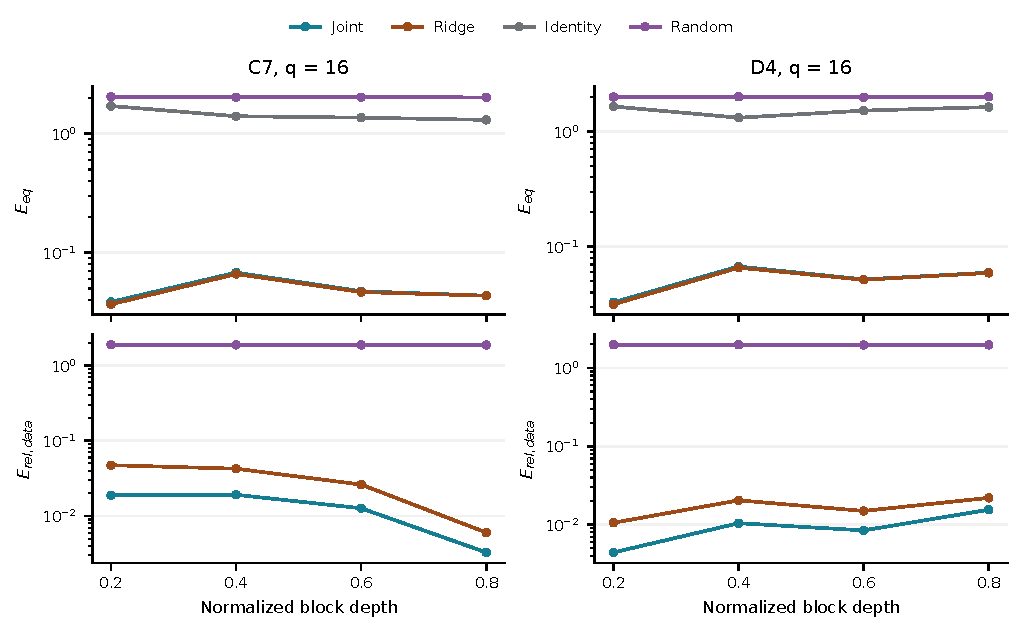
\includegraphics[width=.85\textwidth]{figures/structural_errors.pdf}
\caption{Historical direct prediction and relation consistency across the fixed six-model FULL panel at $q=16$. Joint fitting changes the prediction--consistency tradeoff; the diagnostics do not isolate semantic specificity.}
\label{fig:historical-structural}
\end{figure}
\begin{figure}[t]
\centering
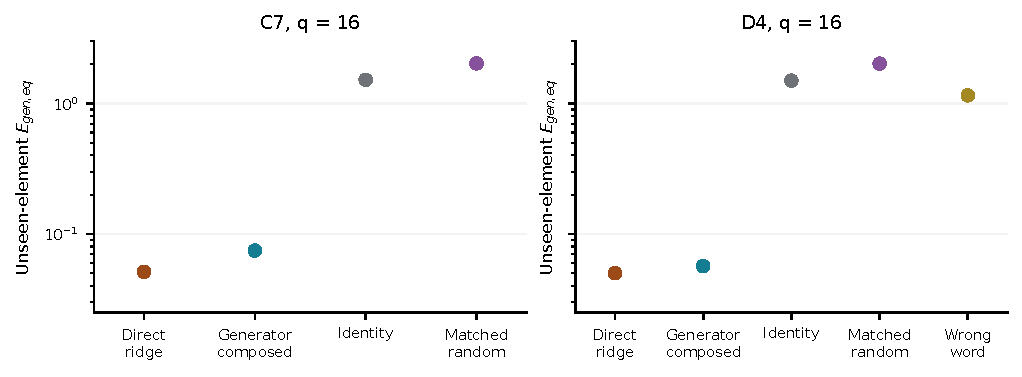
\includegraphics[width=.85\textwidth]{figures/generator_transfer.pdf}
\caption{Generator-only predictions evaluated against transformed held-out activations. Direct element-specific Ridge receives additional supervision. Identity, random generators and wrong words address distinct alternatives. These are the unchanged historical figure values.}
\label{fig:historical-generator}
\end{figure}
Joint relation defects decrease relative to Ridge by $-0.01699$ (recorded 95\% bootstrap interval $[-0.03405,-0.00318]$) for $C_7$ and $-0.00728$ ($[-0.01248,-0.00259]$) for $D_4$. For $D_4$, joint data relation components are $0.01717$ for $r^4$, $0.00876$ for $s^2$, and $0.00320$ for $srs=r^{-1}$. They are approximate relations on activations, not certification of exact ambient representations. In AFS-A, the correct-minus-wrong-word $D_4$ contrast is $-1.097329$ ($[-1.219881,-0.953809]$). All intervals retain the resampling-sensitivity scope of \cref{app:inference}.


The historical FULL joint-minus-random $\Eeq$ contrasts are $-1.9803$ ($[-2.0041,-1.9549]$) for $C_7$ and $-1.9449$ ($[-1.9562,-1.9325]$) for $D_4$. Joint-minus-identity values are $-1.3964$ ($[-1.5882,-1.1982]$) and $-1.4771$ ($[-1.6692,-1.2628]$). These large differences establish useful transformation prediction relative to untrained controls. The more demanding joint-minus-ridge prediction contrasts are slightly positive: $0.001046$ ($[0.000106,0.002285]$) and $0.000864$ ($[0.000149,0.001735]$). Joint-minus-ridge homomorphism differences are $-0.000884$ ($[-0.002083,-0.000018]$) and $-0.000891$ ($[-0.001652,-0.000232]$). These are effects under the historical resampling procedure; their small intervals do not resolve the identification alternatives in \cref{sec:boundaries}.


\begin{table}[h]
\centering
\small
\begin{tabular}{llccc}
\toprule
Group & Estimator & $\Ehom/\Ehomop$ & $\Erel/\Erelop$ & $\Ecomp/\Ecompop$ \\
\midrule
$C_7$ & Joint & 0.00842 / 0.05850 & 0.01348 / 0.09612 & 0.01145 / 0.07879 \\
$C_7$ & Ridge & 0.00930 / 0.06202 & 0.03047 / 0.20903 & 0.01266 / 0.08438 \\
$C_7$ & Random & 1.45937 / 1.03612 & 1.87118 / 1.45048 & 1.98636 / 1.41027 \\
$D_4$ & Joint & 0.00366 / 0.10143 & 0.00971 / 0.17124 & 0.00477 / 0.13149 \\
$D_4$ & Ridge & 0.00455 / 0.11897 & 0.01699 / 0.26283 & 0.00594 / 0.15530 \\
$D_4$ & Random & 1.52346 / 1.08021 & 1.96710 / 1.39203 & 1.98983 / 1.41088 \\
\bottomrule
\end{tabular}
\caption{Recorded primary FULL consistency diagnostics at dimension 16. Data/op pairs deliberately preserve distinct historical metrics: data defects are squared and op defects unsquared; C7 relation aggregands additionally differ. These paired columns should not be read as a comparison on one numerical scale. Homomorphism and composition differ only by excluding identity-containing pairs in the latter.}
\label{tab:full-diagnostics}
\end{table}

\begin{table*}[t]
\centering
\small
\begin{tabular}{lll}
\toprule
Control & Group/metric & Frozen summary \\
\midrule
AFS-B & C7, data homomorphism & 120/120 below reference 2.5th percentile \\
AFS-B & C7, operator homomorphism & 120/120 below reference 2.5th percentile \\
AFS-B & D4, data homomorphism & 120/120 below reference 2.5th percentile \\
AFS-B & D4, operator homomorphism & 120/120 below reference 2.5th percentile \\
AFS-C & C7, state relabel & $-0.577\;[-0.664,\,-0.488]$ \\
AFS-C & C7, target scramble & $-0.596\;[-0.686,\,-0.506]$ \\
AFS-C & D4, state relabel & $-0.765\;[-0.861,\,-0.662]$ \\
AFS-C & D4, target scramble & $-0.729\;[-0.824,\,-0.627]$ \\
\midrule
Global additive & Balanced complete orbit & $\widehat v_g=0$ by permutation cancellation \\
\bottomrule
\end{tabular}
\caption{Registration/correspondence controls and the scope of global additive falsification. AFS-C reports real-minus-scrambled test equivariance error after refitting on perturbed training pairs and scoring against unchanged true held-out targets; negative values favor the real correspondence. Brackets retain the historical bootstrap percentile intervals. AFS-B compares fixed operators with a restricted reference excluding automorphisms; observed and reference registrations are not established as exchangeable, so this is not calibrated semantic-null inference. The global displacement estimator averages complete state orbits and therefore reduces to identity independently of the activations.}
\label{tab:diagnostic-controls}
\end{table*}

AFS-B preserves the fitted matrix family while changing which algebraic element each matrix represents. AFS-C instead changes training correspondence while retaining the activation multiset, refits Ridge and scores it against the true held-out targets. In both groups and both scramble variants, the recorded mean test prediction and data-relation defects increase. The latter are consistency diagnostics on held-out activations, not additional semantic-target accuracy measurements. Prediction error and operator norms are not matched across conditions; moreover, the $C_7$ power-consistency and $D_4$ $srs$ terms normalize by condition-specific fitted outputs. The deterioration therefore does not isolate algebraic fidelity beyond the change in predictive fit. Neither AFS-B nor AFS-C demonstrates that a consistently registered alternative action of comparable learnability would fail.

\subsection{Rank-matched lexical comparison}
\begin{table*}[t]
\centering
\small
\begin{tabular}{lllrrr}
\toprule
Group & Model & Location & $E_{\rm eq}$ & $E_{\rm gen,eq}$ & $E_{\rm rel,data}$ \\
\midrule
C7 & Llama 1B & Embedding & $3.64\!\times\!10^{-6}$ & $5.87\!\times\!10^{-5}$ & $6.37\!\times\!10^{-5}$ \\
C7 & Llama 1B & Internal mean & 0.132327 & 0.198978 & 0.092076 \\
C7 & Qwen 1.5B & Embedding & $2.48\!\times\!10^{-6}$ & $4.25\!\times\!10^{-5}$ & $4.72\!\times\!10^{-5}$ \\
C7 & Qwen 1.5B & Internal mean & 0.171656 & 0.315743 & 0.187296 \\
D4 & Llama 1B & Embedding & $4.97\!\times\!10^{-7}$ & $2.97\!\times\!10^{-6}$ & $3.95\!\times\!10^{-6}$ \\
D4 & Llama 1B & Internal mean & 0.096634 & 0.133246 & 0.051652 \\
D4 & Qwen 1.5B & Embedding & $3.02\!\times\!10^{-7}$ & $1.80\!\times\!10^{-6}$ & $2.39\!\times\!10^{-6}$ \\
D4 & Qwen 1.5B & Internal mean & 0.055191 & 0.059383 & 0.027160 \\
\bottomrule
\end{tabular}
\caption{Rank-matched lexical control using independent Ridge, with generator-only composed predictions for $E_{\rm gen,eq}$. Both locations use C7 $q=6$ or D4 $q=3$; these are not the FULL $q=16$ estimates. Internal means average four fixed depths. Embedding errors are smaller in every tested model/group; all 150 archived internal-minus-embedding intervals are positive. Repeated templates at the embedding location reuse the same category vectors.}
\label{tab:lexical-control}
\end{table*}

\begin{figure}[h]
\centering
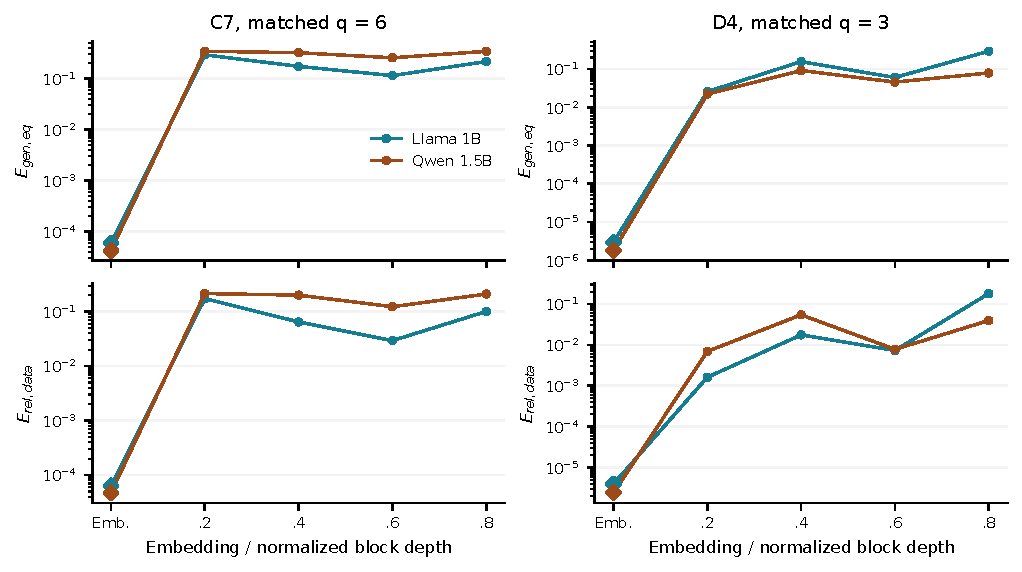
\includegraphics[width=0.76\textwidth]{figures/lexical_internal.pdf}
\caption{AFS-D independent fits at matched lexical ranks: $q=6$ for $C_7$, $q=3$ for $D_4$. This is a two-model comparison and not the dimension-16 primary FULL setting. Lexical near-exactness is compatible with finite-orbit realizability.}
\label{fig:lexical}
\end{figure}
Across the two models and two groups, the internal-minus-embedding contrasts are positive for both prediction and data relation error. This is evidence against internal strengthening in this recorded comparison. It is not evidence that embedding representations encode the uniquely correct semantic action; the full-rank lexical vectors permit every state permutation. Nor does it imply that arbitrary dimensions, models, reading positions, or contextual constructions behave identically.

\subsection{Global additive-field results}
The historical global-field direct errors are additive 1.487859, ridge 0.050149, and joint 0.051104. The additive-minus-ridge contrast is 1.437710 ($[1.400230,1.475673]$), and additive-minus-joint is 1.436755 ($[1.399237,1.474462]$). For repeated C7 generator prediction, the errors are 1.519200, 0.074443, and 0.070297. For the combined D4 paths $r\to s$, $s\to r$, and $s\to r\to s$, they are 1.266128, 0.049265, and 0.047450.

These are the completed experiment's observation-weighted means, not replacements for the FULL or AFS-A primary aggregates. The additive estimator cancels for every action because training covers complete, balanced state orbits. Repeated additive updates therefore cannot track even cyclic motion; for D4, they also cannot distinguish word orders because addition commutes. The reported descriptive order separation is 2.2133 for actual contextual targets, 2.2789 for ridge predictions, and 2.2526 for joint predictions, while the additive prediction has zero separation by construction. The first three are descriptive scores under the recorded normalization, not calibrated accuracies or independent confirmatory tests.

\subsection{Behavioral patching}
\label{app:behavior}
The evaluation prompt appends `` Report the transformed state:'' to a held-out structural prompt. The state remains visible, and the particular transformation is supplied through the selected activation intervention rather than by an explicit textual instruction naming $g$. Let $h$ be the mean state-span hidden vector from this evaluation prompt, $z=(h-\mu)C$, and $C$ the structural training-only PCA basis. The learned replacement is
\[
 h'=h-zC^\top+(zR_g)C^\top.
\]
The forward hook replaces every token position overlapping the state string with this replacement vector at the selected transformer block output, then recomputes the remaining network. If a state occupies multiple input tokens, all overlapping positions receive the same replacement derived from the mean; identity uses the original unpatched output. Thus an identity-matrix patch need not equal the unpatched baseline: overwriting distinct token vectors with their mean can itself change the network. The historical run does not contain a matched zero-delta, token-deviation-preserving sham. The one-token continuation counts below do not establish one-token source spans. These implementation details limit interpretation as a natural state substitution.

The source-conditioned additive comparator is trained from structural training prompts in the original hidden dimension:
\[
 v_{g,i}=\frac1{|\mathcal T_{\rm train}|}\sum_{t\in\mathcal T_{\rm train}}
 (h_{g(i),t}-h_{i,t}),\qquad h'=h+v_{g,i}.
\]
It uses known source-state identity and one vector per element/source pair, so it is more flexible than one source-shared linear operator. Its displacement also acts in the original hidden space, whereas the learned operator changes only the PCA component. The comparison therefore differs in source information, retained parameters and allowed edit subspace. It is an informative stronger comparator because it avoids orbit-averaging cancellation, but it is not a parameter- or subspace-matched test of steering optimality. In the recorded D4 relation rows the additive edit is indexed by the requested target element, so the true word, its direct reference and the wrong-word control receive the same endpoint-conditioned displacement; their equality for this comparator is built into the construction and does not test its composition order.

The target-token score uses the first token of the context-sensitive continuation `` \{target state\}''. Target logit change and target probability change subtract the unpatched prompt's values. The margin is target minus original-state first-token logit, and top-1 success requires the predicted vocabulary argmax to be that target token. The implementation records a full target-sequence log probability only for one-token continuations and would omit multi-token cases for that metric. All archived evaluated continuations contain one token. The scored top-1 outcome therefore concerns that continuation token; this experiment does not test general multi-token answer accuracy.

\begin{table*}[t]
\centering
\small
\begin{tabular}{llll}
\toprule
Group & Metric & Learned minus identity [95\% interval] & Learned minus additive [95\% interval] \\
\midrule
C7 & Target logit & $1.129\;[0.791,\,1.400]$ & $-0.105\;[-0.227,\,-0.014]$ \\
C7 & Top-1 (pp) & $1.743\;[-0.215,\,3.945]$ & $-0.261\;[-1.065,\,0.056]$ \\
D4 & Target logit & $2.406\;[1.932,\,2.833]$ & $-0.007\;[-0.030,\,0.012]$ \\
D4 & Top-1 (pp) & $9.019\;[3.186,\,15.339]$ & $-0.043\;[-0.503,\,0.434]$ \\
\midrule
\multicolumn{4}{l}{D4 correct-minus-wrong final-logit distance: $-0.0422\;[-0.0543,\,-0.0298]$.} \\
\bottomrule
\end{tabular}
\caption{Frozen behavioral contrasts from externally composed activation edits. Additive denotes the training-only source- and transformation-conditioned comparator, distinct from the global additive field. Positive logit/accuracy differences favor the learned edit; the D4 distance contrast is lower for the correct word. Top-1 measures the scored continuation token; all archived continuation counts are one. Recorded 95\% bootstrap percentile intervals preserve the original nested procedure; they describe fixed-panel resampling sensitivity, not calibrated population coverage (\cref{app:inference}).}
\label{tab:causal-main}
\end{table*}

\begin{figure}[h]
\centering
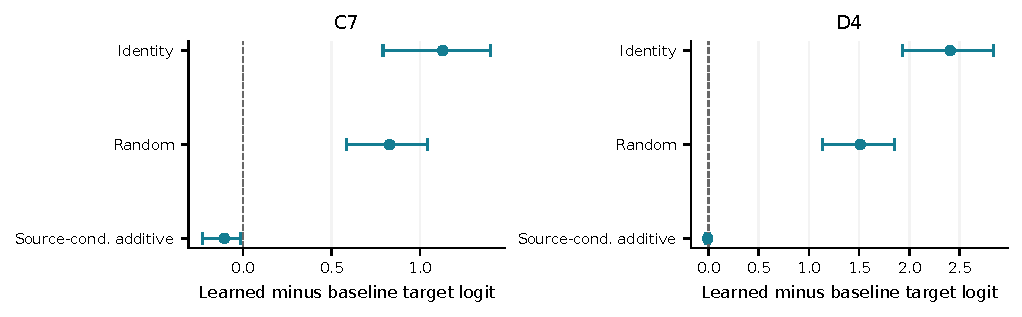
\includegraphics[width=0.76\textwidth]{figures/causal_additive.pdf}
\caption{Learned-minus-source-conditioned-additive target-logit effects. Negative differences favor the stronger additive comparator for that outcome. Directional behavioral effects do not demonstrate causal necessity of a recovered matrix family.}
\label{fig:causal}
\end{figure}
For C7, powers $r^1,\ldots,r^6$ are transformation interventions; $r^7$ is a separate cycle diagnostic. D4 tests $r,s,r^2,r^3$, identity-recovery words $r^4,s^2$, and the relation word $srs$ against a direct $r^{-1}$ intervention. The matched-length wrong word is $rsr$. For final next-token logit vectors $L$, the relation distance is
\[
 d(w,r^{-1})=\frac{\norm{L^{(w)}-L^{(r^{-1})}}_2}{\max(\norm{L^{(r^{-1})}}_2,\epsilon)}.
\]
The historical correct-minus-wrong distance difference is $-0.04220$ ($[-0.05426,-0.02981]$). Both words are evaluated relative to the same direct learned reference; this is an order-sensitive downstream consistency diagnostic, not comparison with a unique ground-truth causal mechanism. The C7 learned-minus-identity target-logit gain is 1.129 ($[0.791,1.400]$), and learned-minus-random is 0.828 ($[0.585,1.041]$). C7 top-1 evidence is weak. Learned-minus-additive target-logit intervals favor the additive baseline in C7 and include zero in D4. Together these observations support behavioral relevance with substantial causal ambiguity. Calendar interventions and competing group-operation mechanisms already demonstrate why an editable representation need not identify native computation \citep{engels2025notall,wu2025unified,feucht2026arithmetic}; the same caution applies to the externally composed edits here.

\FloatBarrier
\subsection{Cross-model compatibility}
Nine fixed pairs comprise all three within-Llama pairs, all three within-Qwen pairs, and size-matched cross-family pairs (1B/1.5B, 3B/3B, 8B/7B). For systems $R_A,R_B$, a row-coordinate map $T$ is assessed through
\[
 R_A(g)T\approx TR_B(g).
\]
The implementation writes $T=P^\top$, stacks the linear constraints $PR_A(g)^\top-R_B(g)^\top P$, takes the smallest right-singular-vector solution, and normalizes $\norm{P}_F=1$. It does not require $P$ to be invertible, well-conditioned, orthogonal, or high effective rank. The normalized score is
\[
 \frac{\mathbb{E}_g\norm{PR_A(g)^\top-R_B(g)^\top P}_F^2}
 {\mathbb{E}_g\norm{R_B(g)^\top P}_F^2+10^{-12}}.
\]
Comparators include an orthogonal Procrustes map estimated from registered activation correspondence, random orthogonal maps, and shuffled group labels. The Procrustes map is fitted on the reported test-template activation pairs and optimizes activation reconstruction, while the intertwiner optimizes commutation using the same group elements later scored. This is a descriptive comparison of two fitting criteria, not predictive transport to unseen paired activations or held-out elements. A low-rank common subspace may suffice. The shuffled-label control keeps the map fitted under true labels rather than refitting after shuffling; it tests sensitivity of that map to registration, not the best achievable fit under each alternative. Shuffled-label controls can also be near-degenerate.

Unlike implementation-family comparisons based on causal abstractions and Congruity \citep{sun2026tracking}, this experiment neither samples behavior-preserving implementations nor estimates their abstraction-dependent distance. The recorded fitted-minus-Procrustes residual differences range approximately from $-0.065$ to $-0.168$ over the registered strata, with historical intervals below zero. This establishes existence of lower-residual fitted commutation maps than the chosen geometry alignment on these elements, not cross-model representation equivalence. The recorded Spearman association with conventional linear CKA is $-0.014$ with interval $[-0.300,0.287]$, leaving that relationship unresolved.

\subsection{Completed controls and remaining identification scope}
The characterization supplies state-centroid, residual and input-only field comparisons under its own sampling and normalization contract. The returned extension additionally completes full-data compact nonlinear predictors, coherent alternative registration, direct context-difference fits and peer adaptations (\cref{app:reproduction}). Their descriptive results are now part of the evidence; they do not retroactively repair a historical comparison's information or intervention mismatch.

The remaining gaps concern stronger claims than the fixed-panel predictive account retained here: algebraic evidence beyond prediction would require a direct-error- and operator-norm-matched comparison; cross-vocabulary generalization would require genuinely new lexical realizations and independently authored context families; native causal use would require competent-task counterfactual evidence. Native confirmation remains blocked despite completed secondary adaptations. None of those stronger claims is inferred from the present comparisons. Future method selection on the inspected holdout would be exploratory and would need fresh evaluation before confirmation. A same-order wrong-group comparison also requires a feasible matched action: no four-state permutation has order eight, so $C_8$ cannot act faithfully on the four corners. An impossible alternative is not an error-matched semantic reference.

\section{Completed Descriptive Characterization}
\label{app:characterization}
The separate study \texttt{icml2027-characterization-v1} was frozen after excluded development comparisons. It completed 72 model/readout/domain cells, 120 legacy split records and 48 $C_7/D_4$ field-comparison cells. Original flags retain \texttt{paper\_eligible=false}, disabled formal inference and no native run. The present manuscript includes manually reviewed descriptive aggregates under a separate provenance record; it does not relabel those flags or the earlier failed gates. The full evaluation is now accessed and cannot serve as an untouched test for subsequent method selection.

\paragraph{Data and information conditions.}
The same six pinned base models and four readouts use training-only $q=16$ coordinates, with BF16 model extraction and F64 coordinate analysis. New extraction comprises 41,728 rows per model: 896 $C_7$, 512 $D_4$ and 40,320 $S_3$ rows, including separately charged support. The C7/D4 state vocabularies are seen in construction. S3 also retains its six abstract assignment states, but its new-entity and joint strata hold out entity names/triples. Unseen-composite supervision concerns actions, not new C7/D4 states or independently authored grammar roots. Coordinate fields receive source coordinates and the requested action. The separate decoded-centroid benchmark has training state labels and the known action table, but decodes the source at evaluation. In contrast, the legacy prediction contrasts in \cref{tab:characterization-intervals} select oracle-source category/retention controls (and an input-metadata potential for S3) on validation; they are not the decoded-source benchmark.

\paragraph{Losses and aggregation.}
The characterization normalizes squared errors by common training-only energy scales; the historical $D$ in \cref{eq:D} averages per-row target-normalized errors. Values across the two studies are therefore not interchangeable. Writing $\bar z_{\rm tr}$ for the training mean, prediction uses $E_z=\mathbb{E}_{\rm tr}\norm{z-\bar z_{\rm tr}}_2^2$. For two paraphrases ordered by their registered identifiers, set $u=z_{p_0}-z_{p_1}$; transport uses $E_u=\mathbb{E}_{\rm tr}\norm{u}_2^2$, without recentering. The row losses are $\norm{\widehat z_g-z_{g(i)}}_2^2/E_z$ and $\norm{\widehat u_g-u_{g(i)}}_2^2/E_u$. Validation and evaluation retain only changed-state pairs $g(i)\ne i$. All-element fitting still uses all training pairs, including identity/fixed points; generator fitting and selection use only primitives. Historical nonidentity-action averages can include D4 fixed points. Prediction and transport thus differ in denominator as well as target. Models and readouts form a fixed panel, averaged within family/entity units. The resampling units are $64\times1$ for $C_7/D_4$, $64\times16$ for jointly new $S_3$ contexts/entities, $64\times24$ for new contexts, and $48\times16$ for new entities. Independently resampled family/entity indices give the crossed $S_3$ sensitivities. No new superiority, equivalence or multiplicity-controlled decision is made.
\begin{table}[htbp]\centering\small
\begin{tabular}{llrrr}\toprule
Domain / split & Endpoint & Baseline minus linear & Lower & Upper \\
\midrule
$C_7$, new context & prediction & -0.002887 & -0.003290 & -0.002495 \\
$C_7$, new context & context & 0.011485 & 0.009997 & 0.013087 \\
$D_4$, new context & prediction & 0.019612 & 0.014730 & 0.025945 \\
$D_4$, new context & context & 0.060918 & 0.049883 & 0.072920 \\
$S_3$, context & prediction & -0.000487 & -0.000791 & -0.000249 \\
$S_3$, context & context & 0.000177 & 0.000010 & 0.000348 \\
$S_3$, entity & prediction & 0.000673 & 0.000443 & 0.000927 \\
$S_3$, entity & context & 0.000739 & 0.000542 & 0.000978 \\
$S_3$, joint & prediction & 0.000460 & 0.000262 & 0.000673 \\
$S_3$, joint & context & 0.000154 & -0.000017 & 0.000338 \\
\bottomrule\end{tabular}
\caption{All ten original characterization contrasts with frozen 95\% percentile sensitivity intervals (10,000 draws, seed 314159). Positive favors linear. Prediction uses oracle-source category/retention controls, plus the $S_3$ input-metadata potential, selected on validation; context uses scalar retention. Prediction and context have different training-energy denominators. Fixed-panel sensitivities do not certify significance, equivalence, coverage or an old power gate.}
\label{tab:characterization-intervals}\end{table}


\paragraph{Prediction and compact category controls.}
All-element direct ridge versus full-kernel means are $0.014900/0.004626$ for $C_7$ and $0.041349/0.020916$ for $D_4$. A training-centroid displacement predictor uses
\[
 \widehat z_g=z+\mu_{g(\widehat i(z))}-\mu_{\widehat i(z)},
\]
where $\widehat i$ is the nearest training centroid. Source decoding is perfect in all $C_7/D_4$ field conditions. C7's error is $0.012013$, better than ridge on average but in only 9/24 individual conditions; D4's $0.062349$ is worse on average and improves only 2/24. Centroids occupy 112 and 64 floating-point coordinates, respectively, plus the exact integer action table and decoding logic. This is a strong cheap control under additional construction labels, not a strict match to label-free field information. Evaluating a known composite label after one source decode is also distinct from repeated primitive evaluation with re-decoding at each intermediate output; the former cannot certify the latter.

\begin{figure}[t]\centering
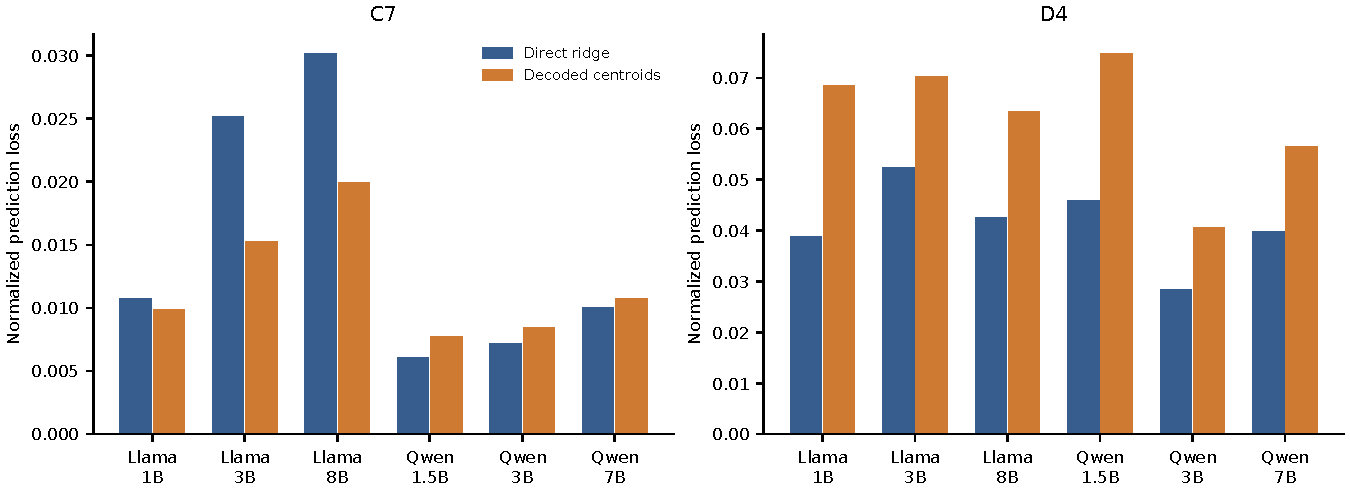
\includegraphics[width=.95\textwidth]{figures/characterization_baselines.pdf}
\caption{All-element prediction: four-readout means for six fixed models. The C7 mean comparison favors decoded centroids in the three Llama models and ridge in the three Qwen models; D4 favors ridge on all six model means. These identities are not independent draws from model lineages. The category comparator has training labels and a known action table. Common PCA and runtime costs are excluded from incremental predictor coordinates.}
\label{fig:characterization-baselines}\end{figure}

\paragraph{What the storage curve measures.}
Primitive-only full fields use 21,504 versus 256 retained coordinates for C7 and 18,432 versus 512 for D4 (84 and 36 times). At the small prescribed budgets they use 256 versus 256 and 480 versus 512. Thus D4 is near-budget, not exactly equal. Farthest-first support selection sees all construction source coordinates but retains only $K$ paired displacements; linear regression compresses all construction target pairs into its coefficients. This original comparison did not fit a compressed nonlinear estimator to all target pairs. The completed RFF/Nystr\"om extension in \cref{app:reproduction} now makes that comparison at explicit parameter budgets; its changed-state/identity handling and selection contract are kept separate from these original values. All 48 full primitive bandwidth selections hit the smallest frozen candidate, $0.125$; some reduced-support selections use $0.25$. These facts bound the comparison and motivate a future development-only grid extension, not retrospective test tuning.

All-element stored ridge maps include an avoidable identity matrix: counts are 1792/2048 for C7/D4, or 1536/1792 after deterministic identity handling. Their $K=14$ fields store 1792/2016, or 1568/1792 after removing zero identity-displacement arrays. C7's original nominal match becomes slightly above-budget after pruning. The common PCA center/basis costs $d(q+1)$ stored float64 coordinates in this export. Training memory, model weights, group tables, centroids, biases, normalization, temporary copies and actual precision must be counted separately for a deployment claim. Retained-coordinate counts are neither total RAM nor statistical capacity.

\paragraph{S3 and context limitations.}
Joint S3 identity prediction loss is $0.018939$, compared with ridge $0.018642$; a small absolute loss is not by itself strong action recovery. The joint context-difference contrast spans zero, and the remaining effects are small relative to the original $0.01$ practical margin. Support displacement reduces prediction loss to $0.015282$ jointly and $0.017580$ on new entities using four extra contexts per entity/state; it is not zero-shot operator superiority. Potential controls were selected in 10/24 conditions (30 split records). Their neural optimization has not been independently replayed. The analytic context fit is separate from that potential. No S3 coordinate-kernel, native intervention or cross-model comparison was added to this original characterization. The subsequent context-predictor and secondary extensions are separately identified in \cref{app:reproduction}.

\paragraph{Audit and provenance boundary.}
The returned archive's checksum, 490-member identity, source/configuration pins, model/readout grid, full metadata banks, exported geometry and 56 frozen intervals were verified. New independent NumPy refits and broader analytic replay reproduced supported coordinate calculations to numerical precision. Historical S3 development selection retains 9,216 reserved cross-block rows per model; exact identities and fitting/scoring masks were checked rather than accepting arbitrary reserved data. The public workflow now validates this historical bank explicitly. Input-feature preprocessing can enumerate nontraining source metadata while assigning zero fitting weight outside training; this is not fitting held-out targets.

The original characterization and its later computational replay are not two independent samples. Compact exports cannot prove original forwards, raw-to-PCA fits, omitted repeated embedding equality or universal prior-access history. Neural Joint/potential refits remain conditional. These limits are recorded with original archive/source hashes and derivative identities in the accompanying release.

\section{Returned Computational Replay and Completed Extensions}
\label{app:reproduction}
The returned run re-executes previously inspected historical and characterization designs and evaluates the previously specified compact/context and secondary extensions. It is a computational reproduction with preserved scientific stops. It does not supply an independent test of the historical claims or convert the failed native protocol into a successful causal study. Original \texttt{paper\_eligible=false} and \texttt{independent\_confirmation=false} records remain unchanged; the tables here are explicitly reviewed descriptive derivatives. All model/readout conditions are retained rather than selecting a favorable subset.

\subsection{Completed scope and preserved stopping decisions}
\begin{table}[t]\centering\small
\caption{Final returned execution status. ``Complete'' concerns the named computation; scientific eligibility is separately stated. No absent confirmation result is imputed from a completed secondary branch.}
\label{tab:reproduction-status}
\begin{tabular}{p{.31\textwidth}p{.61\textwidth}}\toprule
Component & Recorded outcome and interpretation \\\midrule
Historical FULL/PRE-FULL & Complete; archived computations agree with the previous frozen tables. \\
AFS A/B/C and additive extensions & Complete under their historical definitions; pass labels do not exclude all category/context explanations. \\
Original $q=16$ embedding AFS-D & Infeasible: centered lexical training rank is six in the failing weekday cell. Original failed unit retained. \\
Separate rank-aware AFS-D & Complete at $q=6$ for $C_7$ and $q=3$ for $D_4$; embedding-dominant diagnostic, not a replacement $q=16$ pass. \\
Original synthetic calibration & Stopped: recorded Y4 sensitivities $0.870$ ($C_7$) and $0.825$ ($D_4$) are below $0.90$. \\
Revised BF16/F64 calibration & Complete; passed its specified synthetic-generator criteria. \\
Characterization / compact--context & Complete; 72 coordinate cells / 240 component--registration jobs. Descriptive analyses of inspected designs. \\
Structural power & Limited precision; no selected family count or overall powered-confirmation claim. Separate $S_3$ planning target met. \\
Pilot / native preparation & Stopped: first $m_0.C_7$ clean accuracies are $0.0625$ development and $0.15625$ transfer, below $0.80$. \\
Structural / native confirmation & Blocked by their scientific dependencies; no confirmatory outcomes. \\
Peer, cross-model, product, interface & Complete as separate secondary diagnostics; their scopes are detailed below. \\
\bottomrule\end{tabular}
\end{table}

The native stop concerns the registered program task and endpoint. Shorter or differently prompted development diagnostics cannot substitute for its gate. Likewise, a synthetic calibration pass assesses the specified decision procedure under simulated regimes; it does not certify a native mechanism. The structural power record retains \texttt{limited\_precision\_do\_not\_claim\_powered}. A separate $S_3$ planning calculation selects 64 families and 16 orbits, without overriding the blocked overall confirmation.

\subsection{Compact nonlinear predictors and coherent registration}
The compact extension reads the completed $q=16$ coordinate banks with unchanged training, validation and test roles. It includes independent linear and affine ridge, decoded-centroid displacement, limited-support Gaussian fields, random Fourier feature residual regression, and Nystr\"om residual regression. The last two fit all construction target pairs at each budget. Training-source landmarks, feature parameters, normalizers, coefficients, biases and numeric lookup tables are charged to incremental float64/int64 parameter storage. Shared PCA, model weights, temporary arrays and Python/runtime overhead are excluded. Logical parameter bytes are not compressed file size, total RAM or a statistical-capacity equivalence.

\begin{table}[htbp]\centering\small
\begin{tabular}{lrr}\toprule
Method & $C_7$ & $D_4$ (corners) \\
\midrule
Ridge & 0.01490 & 0.04192 \\
Decoded centroid & 0.01201 & 0.06382 \\
Limited support, $1\times$ & 0.66133 & 0.49167 \\
RFF, $1\times$ & 0.30033 & 0.21265 \\
Nystr\"om, $1\times$ & 0.08292 & 0.04942 \\
\bottomrule\end{tabular}
\caption{All-element changed-state prediction in the reviewed replay: equal action then equal cell means over 24 fixed model/readout cells per group; lower is better. $1\times$ denotes nominal incremental storage relative to ridge, not equal capacity or total RAM. Centroids additionally use construction labels and an action table. All budget and registration results are retained in the release.}
\label{tab:reproduction-compact}\end{table}

\begin{table}[htbp]\centering\small
\begin{tabular}{llrrrrr}\toprule
Group & Estimator & $0.5\times$ & $1\times$ & $2\times$ & $4\times$ & $8\times$ \\
\midrule
$C_7$ & Limited support & 0.76776 & 0.66133 & 0.65234 & 0.64495 & 0.64310 \\
$C_7$ & RFF & 0.93529 & 0.30033 & 0.06631 & 0.01174 & 0.00708 \\
$C_7$ & Nystr\"om & 0.49296 & 0.08292 & 0.01243 & 0.00845 & 0.00612 \\
$D_4$ & Limited support & 0.52597 & 0.49167 & 0.48148 & 0.47483 & 0.47389 \\
$D_4$ & RFF & 0.63453 & 0.21265 & 0.06644 & 0.02778 & 0.02229 \\
$D_4$ & Nystr\"om & 0.17035 & 0.04942 & 0.03153 & 0.02333 & 0.01960 \\
\bottomrule\end{tabular}
\caption{All five declared nominal budgets for the all-element semantic track, equal action then equal cell means over 24 cells. This table does not choose a budget on the inspected test set. Generator-only and coherent-action results remain separate in the machine-readable release.}
\label{tab:reproduction-budgets}\end{table}

Fixed budgets are $0.5,1,2,4,8$ times the identity-pruned linear reference (\cref{tab:reproduction-budgets}). The all-element and primitive-only tracks have different supervision. Primitive composition repeatedly applies each predictor to its own output, including repeated source decoding for centroids. Infeasible budget conditions and invalid predictions remain explicit. Validation selects the prescribed candidates without using test targets; all budgets and all cells remain in the released summaries. \Cref{tab:reproduction-compact} reports the fixed unit-budget all-element comparison rather than a test-selected operating point. The complete curve shows that Nystr\"om improves mean error over ridge at $2\times$ and RFF at $4\times$ storage in both groups. This descriptive operating-point comparison is distinct from a validation-selected deployment policy; selecting a budget retrospectively on these test means would require new evaluation.

The decoded-centroid control receives construction state labels and an exact group-action table, beyond source-coordinate/action access. Its unit-budget all-element means are $0.012013$ and $0.063821$ for $C_7/D_4$, versus ridge $0.014897$ and $0.041919$. With primitive-only fitting, generator-composed means over all nonidentity actions are $0.012013/0.063821$ for centroids and $0.021114/0.045896$ for ridge. The unit-budget Nystr\"om means on that track are $3.643199/0.087822$; a good direct predictor need not yield stable repeated composition. This all-action aggregate includes the fitted generators and must not be described as an unseen-element-only endpoint. These are descriptive means, without a claim that the selected nonlinear designs exhaust the alternative class. They must not silently replace the original characterization's related but distinct fitting/identity-handling tables.

Every action is also conjugated by the fixed state swap $(0,1)$ to define a coherent alternative registration. The alternative preserves group laws and fixed-point counts and uses the same supervision format and fitting procedure, applied to its own consistent target correspondence. All-element ridge means are $0.017503/0.041871$ for this registration, versus semantic $0.014897/0.041919$. Both use the same underlying source bank and abstract action labels, but targets and changed-state evaluation masks are registration-specific. The $D_4$ scored rows can differ because conjugacy preserves fixed-point counts without fixing their identities; this is not an identical-row, identical-target comparison. One conjugate reference is neither an exhaustive comparison with all finite actions nor an exchangeable randomization test. A validation-only comparability ledger retains both matched and unmatched conditions under the fixed 1.25 factor for error and output squared norm, plus linear coefficient norm where available. This does not match nonlinear Jacobian norms.

\begin{table}[htbp]\centering\small
\begin{tabular}{lrr}\toprule
Method & $C_7$ & $D_4$ (corners) \\
\midrule
Ridge & 0.023180 & 0.048802 \\
Decoded centroid & 0.012814 & 0.066672 \\
Limited support, $1\times$ & 1.547945 & 0.899571 \\
RFF, $1\times$ & 3.040965 & 0.390158 \\
Nystr\"om, $1\times$ & 4.304052 & 0.095135 \\
\bottomrule\end{tabular}
\caption{Generator-only fitting evaluated solely on the five excluded nonidentity elements in each group. Equal action means precede equal means over 24 cells. The unit storage budget now refers to generator matrices. These numbers are distinct from the all-nonidentity evaluation, which includes fitted generators. No new model or predictor was fitted for this aggregation.}
\label{tab:reproduction-unseen}\end{table}

The separate excluded-element endpoint in \cref{tab:reproduction-unseen} removes the fitted generators before averaging. It is computed from the original saved per-action records, with no predictor refitting.

\subsection{Context-difference transport}
\begin{table}[htbp]\centering\small
\begin{tabular}{lrrr}\toprule
Method & $C_7$ & $D_4$ (corners) & $S_3$ (joint) \\
\midrule
Identity & 0.045755 & 0.181386 & 0.016444 \\
Coordinate-fitted operator & 0.047137 & 0.132304 & 0.016298 \\
Context-fitted linear & 0.034260 & 0.116386 & 0.016290 \\
Oracle category retention & 0.043825 & 0.166675 & 0.016313 \\
Context-fitted, coherent action & 0.034465 & 0.117165 & 0.016291 \\
\bottomrule\end{tabular}
\caption{Context-difference transport on 24 fixed cells per stratum. Coherent swap01 defines a consistently relabeled alternative action; it is not an exchangeable semantic null. Each registration uses its own targets and changed-state mask; retained D4 pairs need not coincide. All predictors within one registration share its scoring rows. The context loss uses its own training-energy normalization, not the coordinate-prediction denominator.}
\label{tab:reproduction-context}\end{table}

For registered paired paraphrases, the source is $u_i=z_{p_0,i}-z_{p_1,i}$ and the target is $u_{g(i)}$. The uncentered training difference energy supplies a common denominator for these comparisons; it differs from coordinate prediction energy and historical per-row normalization. The extension compares identity, per-action scalar retention, coordinate-fitted operators, directly fitted linear difference maps, full-data RFF/Nystr\"om difference regressors, and category-retention controls. The decoded-category arm additionally receives the paired source center; the oracle arm additionally receives the true category. These information advantages remain labeled. Within each registration, the compared predictors share targets and the changed-state mask. Across registrations, targets differ and retained $D_4$ pairs need not coincide. $S_3$ new-context, new-entity and joint strata are separate; reserved/support rows do not enter primary fitting or selection.

Dedicated linear difference fitting improves the mean $C_7/D_4$ transport error relative to applying coordinate operators to the differences. The fixed coherent registration yields $0.034465$, $0.117165$ and $0.016291$ for $C_7$, $D_4$ and jointly new $S_3$, close to the semantic means in the table. These context scores also use each registration's own changed-state mask, including potentially different D4 rows. Thus the result supports a distinction between fitting objectives, while leaving semantic specificity unresolved. The $S_3$ joint difference from identity is much smaller than the inherited $0.01$ practical margin; no new power or equivalence decision is assigned from these descriptive means.

\subsection{Constructively trained interfaces}
\begin{table}[htbp]\centering\small
\begin{tabular}{lrrrr}\toprule
Objective & $C_7$ loss & $D_4$ loss & $S_3$ joint loss & $S_3$ joint acc. \\
\midrule
Reconstruction & 0.212166 & 0.244488 & 0.410680 & 0.1657 \\
Orbit augmentation & 0.212144 & 0.244781 & 0.410358 & 0.1659 \\
Equivariance & 0.229303 & 0.254190 & 0.401808 & 0.1671 \\
Group regularization & 0.227646 & 0.253783 & 0.401694 & 0.1671 \\
\bottomrule\end{tabular}
\caption{Validation-selected supervised interfaces: 72 model/readout/seed cells per objective and domain, 500 steps per candidate. The loss is normalized full-hidden target-prediction error; it is not the compact-coordinate endpoint. State classification is an interface-head score, not language-model answer accuracy. Seed replicates are not independent datasets.}
\label{tab:reproduction-interface}\end{table}

The interface extension trains supervised rank-16 encoder/decoder/operator systems on the high-dimensional construction activations. It compares reconstruction, complete-orbit augmentation, equivariance consistency and group regularization. There are 1,728 candidate parameter checkpoints, 500 training steps each, with technical seeds 101, 303 and 909; validation selects 864 arm/seed/cell fits. Each domain's table averages 24 model/readout cells and three seeds. All saved candidates, including unselected regularization weights, remain available.

Adding group regularization does not improve mean full-hidden target prediction over reconstruction for $C_7$ or $D_4$, despite nearly perfect transported-state classification. For $S_3$, the modest prediction improvement accompanies classification near $1/6$ on new entities and joint strata; new-context classification is also weak. This is a constructed supervised interface, not evidence that the unchanged language model uses the learned operators. The high-dimensional training-energy-normalized loss is distinct from the compact-coordinate metric. Equal step counts do not establish equal information, capacity or total computation.

\subsection{Peer adaptations and cross-model/product diagnostics}
\begin{table}[htbp]\centering\small
\begin{tabular}{llrr}\toprule
Task & Method & Error & Conditions \\
\midrule
Word & Procrustes & 3.10155 & 60 \\
Word & Ridge affine & 0.42475 & 60 \\
Word & Hu Eq.~12 (source displacement observed) & 0.52642 & 60 \\
Structural & Procrustes & 7.43045 & 48 \\
Structural & Ridge affine & 0.27236 & 48 \\
Structural & Constrained intertwiner & 0.99194 & 48 \\
$C_4\times C_4$ & primary operator & 0.06035 & 24 \\
$C_4\times C_4$ & joint & 0.07267 & 24 \\
$C_4\times C_4$ & local displacement & 0.00539 & 24 \\
\bottomrule\end{tabular}
\caption{Secondary fixed-panel summaries. Word and structural transport use row-normalized errors; the product endpoint has its own target-energy normalization. Values across tasks are not directly comparable. The Hu adaptation receives source-model test displacements. These are implemented adaptations, not certified peer-author reproductions.}
\label{tab:reproduction-secondary}\end{table}

The peer factorial branch fits conditional-mean/ANOVA tables on construction grids. It retains 76,800 unique recipient/condition scores: 15,360 validation and 61,440 test scores, covering two base models, $C_7$ and the free-eight-state $D_4$ task. Eight conditions combine state/operation/joint edits with full-hidden or matched-subspace support, a three-way ablation and a zero-delta sham. This is an Arora-inspired task adaptation, not verified execution of the authors' code. Zero-delta test generation accuracy is only $22.10\%/1.03\%$ for Llama $C_7/D_4$ and $19.59\%/15.63\%$ for Qwen. The branch therefore supplies diagnostic measurements under poor native competence, not a competent-task causal efficacy certification. Different-target edit and sham accuracies cannot be subtracted as if they measured an identical answer endpoint.

The Engels/Wurgaft anchors record \texttt{author\_code\_executed=false}; exact author commits, prompts and layer equivalence are uncertified. Their aggregate accuracies ($0.07143$, $0.09184$, $1.0$) pertain to different prompts and method mixtures. They neither reproduce published leaderboard entries nor replace the failed longer-program competence test. No peer-superiority claim is made from these aggregates.

Word transport covers 60 conditions; structural transport covers 48. Hu-style transport receives source-model test before/after displacements, an additional information condition. Ridge-affine has lower average error than this implementation on the word panel. On the structural panel, the constrained intertwiner has error $0.99194$ and mean residual cosine $0.07384$, versus ridge-affine error $0.27236$. Its constrained compatibility fit is not generally successful predictive transport or a Congruity test. The $C_4\times C_4$ product task adds 24 cells, but local displacement ($0.00539$) improves substantially on primary linear ($0.06035$) and Joint ($0.07267$) prediction. Domain extension is therefore distinct from general operator superiority.

\subsection{Integrity, numerical replay and remaining verification limits}
All 567,055 returned ZIP members pass CRC/decompression and SHA256 checks, including the export manifest. The source manifests match the preserved release. The 3,573 FULL/PRE-FULL artifacts shared with the earlier returned archive are unchanged. All 240 compact/context payload identities and all paired interface parameter hashes verify; saved parameter arrays are finite, and all 864 interface selections match their registered validation minimum and tie-break. These checks establish storage/selection consistency, not independent retraining.

Historical comparison matches all 1,193 rows in five frozen interval tables, with maximum estimate/endpoint difference approximately $4.44\times10^{-15}$. Independently executing five representative complete coordinate analyses---Qwen2.5-1.5B layer 11, $C_7$ and $D_4$ compact/context plus $S_3$ context---matches 173,314 numeric leaves at relative tolerance $10^{-7}$ and absolute tolerance $10^{-9}$. Maximum absolute difference is approximately $1.42\times10^{-6}$. This is tolerance-level agreement for those complete analyses, not bitwise equality or an independent numerical replay of all 240 jobs.

The archive intentionally omits raw hidden-state caches and model weights. It therefore supports the reported compact refits and saved-result audit, but does not itself re-verify raw-to-PCA fitting, every pretrained forward or every high-dimensional interface fit. Recorded model/source pins support rebuilding those inputs. Failed calibration, infeasible rank, competence stops and blocked branches remain evidence. A computational replay of inspected designs cannot increase the number of independent scientific replications.

\section{Prospective Identification and Native-Task Evaluation}
\label{app:prospective}
This appendix preserves the original identification/native protocol and distinguishes the subsequent characterization amendment. Historical FULL/AFS evidence, excluded development analyses and subsequent descriptive outcomes have different evidential roles.

\paragraph{Completed characterization and replay (24 October 2026).}
The revised BF16/F64 synthetic calibration completed, while the original calibration failure remains recorded. The excluded pilot completed structural eligibility and power calculations; structural power remained limited and native preparation stopped at clean competence. The separate \texttt{icml2027-characterization-v1} study was frozen after excluded development work. Its results were subsequently inspected and manually summarized descriptively. Reproducing those computations does not restore an untouched test set or establish independent confirmation.

The returned reproduction additionally completes the fixed compact/context panel, rank-aware historical continuation, peer adapters, factorial comparisons, word and structural cross-model transport, product actions and constructive interfaces (\cref{app:reproduction}). These branches have distinct inputs and evidential roles. Their completion neither overrides the native competence stop nor authorizes the blocked confirmation branches. The original characterization remains identifiable: it did not itself include these later extensions. Original output flags, failed units, numerical tables and source identities are preserved; reviewed derivative tables have separate provenance.

The characterization uses the six pinned base models, four readouts and training-only $q=16$ PCA. Its family/crossed 10,000-replicate percentile intervals (seed 314159) describe sensitivity of a fixed panel; they are not new multiplicity-adjusted hypothesis tests or model-population confidence statements. The completed compact/context extension reports descriptive fixed-panel means without new significance decisions. Verification covers archived integrity, stored selections, historical numerical agreement and representative analytic refits. Raw pretrained forwards, raw-to-PCA fits and complete neural retraining are outside that local verification. No further calibration or full rerun is required to report the completed evidence.

\subsection{Original identification and native protocol (retained scope)}

\paragraph{Sampling and partitions.}
The default structural study uses 48 training, 16 validation and 32 test scenario families, with two paired paraphrases per family and 12 additional pilot families. A declared compositional generator samples scenarios under a fixed collection of grammar roots; this supports inference conditional on that generator, not a claim of 96 independently authored grammars. External authored banks can be imported with family and grammar-root identities. A maximum candidate test pool is sealed before pilot analysis; prospective power selects a prefix of 32, 48 or 64 families before its activations are collected. The maximum pool also contains 24 new entity triples; crossed power selects 16 or 24. All states of a scenario remain together. Per-root and leave-one-root-out summaries assess sensitivity to the fixed grammar generator; they do not establish transfer to independently authored grammars. The six historical checkpoints and four relative depths are fixed conditions rather than independent model-population draws.

\paragraph{New entity transfer.}
Alongside $C_7$ and the historical four-corner $D_4$ task, an $S_3$ role-binding task crosses scenario families with 48 disjoint entity triples, split 24/8/16. Each triple has six assignments. Training uses training-family by training-triple cells; validation uses validation by validation. The principal transfer block contains new families and new triples. A single fixed final-token readout measures the complete clause; concatenating role-aligned hidden vectors would engineer the desired action and is excluded from the primary measurement. Zero-shot evaluation uses no target-triple activation centroids. A separately charged equal-support arm provides four disjoint support contexts per assignment state to all applicable methods.

\paragraph{Strong alternative explanations.}
Training centroids $\mu_i$ define $z-\mu_i+\mu_{g(i)}$ and scalar residual-retention baselines. Their state indices update under composition. Oracle-source and construction-decoded-source conditions are separate. Independent linear ridge is the primary prediction procedure; ridge on training context-difference pairs is the co-primary transport procedure. Affine, Procrustes, residual, Joint and validation-selected local-displacement variants are secondary. The local field is evaluated against actual held-out targets and reported separately from the analytic linear-estimator null calibration. Regularization is selected on validation, with penalty $\rho=\lambda\operatorname{tr}(X^\top X)/q$ and a declared grid including a pseudoinverse candidate. The $S_3$ comparison additionally fits a compositional potential field to construction entity embeddings and role metadata, without held-out target activations.

For paraphrases $t,t'$ within family $f$, evaluate transport of $u_i=z_{t,i}-z_{t',i}$ to $v_{g,i}=z_{t,g(i)}-z_{t',g(i)}$, against zero and validation-selected scalar identity transport. Target and difference losses use common training-only energy scales. Low training context energy makes the difference endpoint uninformative and is retained as such. Exact coherent fixed-feature action reassignments provide 120 cyclic image families and three four-corner dihedral image families; the latter has only $1/3$ minimum all-element tail-rank resolution. These structural ranks are not automatically semantic randomization p-values.

\paragraph{Calibration and uncertainty.}
Six disclosed synthetic regimes test category-only realizations, shared context, independent state--context noise, genuinely equivariant interaction, family-specific transport and unsupported ambient extensions. Calibrate the actual fitted-estimator decision rule and distinguish statistical error from semantic nonidentification. The primary $C_7/D_4$ inference aggregates fixed models and depths within each family and uses family-level tests with Holm correction. Its eight superiority/equivalence hypotheses receive familywise level .04; the four zero-shot $S_3$ hypotheses receive .01 and a separately calibrated crossed family/orbit analysis. The proposed normalized superiority margin is .01 and equivalence half-width .005. These are research choices, not conference thresholds. Bootstrap results are sensitivity analyses; overlapping split seeds do not multiply the sample size.

\paragraph{Native computation.}
The causal study starts with Llama-3.1-8B and Qwen2.5-7B, subject to a development-only clean-competence gate. It uses genuine weekday programs and a separate free-eight-state $D_4$ task on an asymmetrically marked square. For prefix $p$, generator edit $g$ and native continuation $v$, the counterfactual answer is $v(g(p(i)))$; a natural counterpart starts from $p^{-1}gp(i)$. The model executes $v$. Externally composing an edit is not described as the model executing those matrices. A candidate intermediate site must carry the proposed variable without inserting its ground-truth answer into the prompt.

For span means $\bar h,\bar h^*$, the primary hook uses $h_j'=h_j+\alpha(\bar h^*-\bar h)$, preserving token deviations and the declared complement. Include zero-delta and historical mean-overwrite shams, natural donors, source-conditioned means, shrinkage, affine/Procrustes/local fields and fixed-seed random carriers. Earlier consumer sites are primary; late patches are positive controls. Select the best trainable baseline on validation. Score complete answers, sequence margins, invalid outputs and collateral effects. The primary accuracy contrast uses held-out continuation words of length six to eight; shorter words remain a separate sensitivity condition. The excluded pilot uses the test panel's long/short allocation. A five-point observed accuracy advantage with an adjusted positive bound is a proposed practical target; it does not establish a unique native algorithm. Operation-only, joint-variable and pathway interventions require their separately defined carriers and tests. A secondary capacity panel fits ranks two, four and eight at the frozen primary sites, with its own construction fits and validation-selected baselines frozen before test outcomes. Rank-two action maps can therefore be compared with the rank-two calendar plane; the primary rank-sixteen test is unchanged.

\paragraph{Peer comparisons.}
Compare calendar-plane interventions \citep{engels2025notall}, conditional-mean relation steering \citep{arora2026causal}, and compatible manifold steering \citep{wurgaft2026manifold} on shared sealed cases. Retain original-setting implementation anchors separately from common-benchmark adaptations. Declare masks, complement preservation, intrinsic rank, supplied labels and tuning budgets. Engels mean-ablates complementary components; Wurgaft preserves the PCA complement in its manifold arm but replaces the full activation in its straight-line comparator. Reproduction and matched-complement adaptation must therefore be reported separately. Full functional ANOVA requires a factorial panel rather than sparse scenario samples. Hu's cross-model transport \citep{hu2026language} receives source-model test-word displacements and belongs in a separately labeled information regime. Global/local action fitting is situated relative to \citet{sun2026transformationlaws}; potentially singular intertwining is not Congruity \citep{sun2026tracking}. Geometry, a predictive carrier and a uniquely used computation are different claims \citep{hindupur2026comparison,makelov2024illusion,zhang2024patching}. Symbol rebinding and group programs also have direct precedents \citep{todd2026algebra}.

\paragraph{Outcome policy.}
Publish negative, infeasible and inconclusive conditions. If category/local baselines explain the effect, limit the structural claim. If only late patches succeed, report a control interface. A native-use interpretation requires prospective counterfactual fidelity and specificity within the tested abstraction. A third training lineage is a preselected replication, not an opportunity to replace unfavorable primary conditions. No unexecuted condition is represented by a numerical result.


\section{Extended Related Work}
\label{app:related-work}
\paragraph{Recovering transformations in existing representations.}
Lenc and Vedaldi \citeyearpar{lenc2015understanding} fit paired linear/affine maps with reconstruction and task losses and study cross-network stitching. Sun \citeyearpar{sun2026transformationlaws} studies compatible transformation families, encoder-fibre/kernel conditions, global/local realizations and error accumulation; its pooled linear-risk decomposition explicitly isolates a sharing cost. Its evaluations distinguish prediction, unseen-start transport, composition, and downstream fidelity in visual features. Action existence and shared-versus-local fitting therefore have direct precedents. Our contribution is the completed comparison of lexical/rank controls, coherent registrations, storage budgets and contextual transport in a fixed LLM panel; the supporting elementary identities are not a new general identification theory.

\paragraph{Calendar representations and their computational use.}
Linear concept geometry and its intervention metric are developed by \citet{park2023linear}, with categorical and hierarchical structure studied further by \citet{park2025categorical}. \citet{engels2025notall} identify multidimensional calendar features and causally patch circular representations in arithmetic tasks; their intervention-based appendix also discusses finite-group computations. Their statistical notion of feature irreducibility is distinct from invariant-subspace irreducibility in group representation theory. \citet{karkada2026emergent} connect language statistics to representational geometry. \citet{feucht2026arithmetic} investigate calendar arithmetic through a computational route involving ordinary addition and subsequent cyclic decoding. Consequently, our weekday experiment neither discovers calendar circles nor establishes a novel calendar-steering mechanism. It measures a particular fitted operator system on a fixed vocabulary and context distribution.

\paragraph{Group-operation mechanisms and competing interpretations.}
\citet{nanda2023progress} reverse engineer Fourier computations for modular addition. \citet{chughtai2023toy} recover representation-theoretic structure in networks trained on group products, while \citet{wu2025unified} develop compact performance proofs for a subset of group-operation networks and show that matching intervention effects need not identify an algorithm. Coset-based explanations \citep{stander2024cosets} and dihedral-multiplication mechanisms \citep{wei2026dihedral} supply further evidence that algebraic structure and noncommutative neural computations predate this work. Unlike those algorithmic tasks, our unchanged pretrained models are not trained by us to output binary group products. Multiplying recovered matrices externally and inserting one resulting activation edit is a different experiment from reverse engineering the unedited model's native multiplication algorithm.

\paragraph{Learning actions and measuring compositionality.}
Equivariance by Contrast \citep{schmidt2025equivariance} jointly learns latent coordinates and action representations from unlabeled action-paired observations. Its identifiability theorem assumes injective mixing, sufficiently diverse/spanning data and exact matching conditional distributions, and recovers coordinates up to one invertible linear map, with correspondingly conjugated actions. Here the encoder, readout and labeled input action are fixed; we assess predictive fits in those coordinates. This observation contract differs from joint latent recovery and does not extend its theorem or transfer its guarantees to our measurements.

Homomorphism autoencoders learn action representations from transitions \citep{keurti2023homomorphism}. \citet{an2026homomorphism} assess compositional generalization with representational homomorphism errors on expression tasks; this is a direct precedent for evaluating hidden representations through composition, rather than a geometry-only comparison. We fit element-indexed transport operators on contextual lexical states and separately test prediction and products. Equivariant architectures \citep{cohen2016group,kondor2018generalization,weiler2019general}, group crosscoders, and equivariant sparse autoencoders \citep{gorton2024group,erdogan2025group} provide related symmetry-aware tools, while making different architectural or dictionary-learning commitments.

\paragraph{Probes, equivalence, and causal evidence.}
Probe selectivity requires controls for the tasks a fitted map can learn \citep{hewitt2019designing}. \citet{yao2026groupaction} emphasize the equivalence relation underlying representation claims; the coordinate-change group in that discussion must not be confused with our semantic input-action group. Exact laws survive conjugacy, whereas the reported approximate Euclidean defects depend on the selected metric. \citet{sun2026tracking} compare implementation families through causal abstractions and Congruity, with explicit assumptions linking representation distances to interpretive equivalence. Our same-element intertwiner is a narrower compatibility fit, not that test. Causal abstraction requires intervention consistency beyond directional score movement, and successful control does not alone identify native reasoning \citep{geiger2022inducing,geiger2025causal}.

\paragraph{Geometry, steering, and fields.}
Word relations, spatial probes, and representational convergence provide broader context \citep{mikolov2013linguistic,bolukbasi2016man,gurnee2023language,huh2024platonic}. Activation and representation engineering \citep{turner2023activation,zou2023representation}, manifold steering \citep{wurgaft2026manifold}, and contextual transformation geometry \citep{hu2026language} motivate behaviorally meaningful transformations. Conditional-mean interaction steering also depends on a factorial construction \citep{arora2026causal}; a state-centroid control is only a restricted adaptation. Our constant global displacement estimator is not a reproduction of these methods. A linear operator itself admits the state-dependent residual form $zR_g=z+z(R_g-\Id)$; the tested distinction is constant displacement versus state-dependent transport, not additive versus algebraic structure in general.


\end{document}
